\documentclass[brudnopis]{xmgr}
\usepackage{amsrefs}
\usepackage{mathtools}
\usepackage{ccaption}
\usepackage{amsthm}
\usepackage{todonotes}
\usepackage{placeins}
\usepackage{enumitem}

\DeclarePairedDelimiter\ceil{\lceil}{\rceil}
\DeclarePairedDelimiter\floor{\lfloor}{\rfloor}
\newtheorem{Twierdzenie}{Twierdzenie}
\newtheorem{Lemat}{Lemat}
\newtheorem{Definicja}{Definicja}

\wersja   {wersja wstępna [\ymdtoday]}

\author   {Jakub Ciechowski}
\nralbumu {186471}
\email    {jakubciechowski@gmail.com}

\title    {Problem galerii sztuki dla odcinków na płaszczyźnie}
\date     {\ymdtoday}
\miejsce  {Gdańsk}

\opiekun  {dr Paweł Żyliński}

\begin{document}
%
%\begin{abstract}
%  Streszczenie…
%\end{abstract}
\keywords{Problem galerii sztuki}

%% tytuł i spis treści
%\maketitle
%
%% wstęp
%\introduction

% \chapter{Klasyczny Problem galerii sztuki}

% \section{Problem galerii sztuki dla wielokątów prostych}

% % idzie do wprowadzenia
% % Jako pierwszy problem galerii sztuki przedstawił Victor Klee w 1973, odpowiadając na prośbę Vaseka Chv\'atala o interesujący problem geometryczny. Zagadnieniem, które zaproponował Klee było znalezienie minimalnej ilości strażników, wystarczających aby strzec wnętrze pomieszczenia galerii sztuki o kształcie n-kąta. Niedługo potem Chv\'atal zaproponował teorię, która szybko została nazwana ,,Teorią galerii sztuki Chv\'atala'', która mówi, że $\floor{\frac{n}{3}}$ strażników jest zawsze wystarczających a czasami potrzebnych aby strzec n-kąt (Chv\'atal 1975). Od tamtego dnia problem doczekał się wielu różnych wariacji oraz przekształceń.

% \subsection{Twierdzenie Chv\'atala (1975)}
% Zgodnie z twierdzeniem Chv\'atala (1975)\label{tw chvatala}, ilość strażników potrzebnych do strzeżenia wielokąta prostego wynosi g(n) $\le$ $\floor{\frac{n}{3}}$, gdzie g(n) jest funkcją opisującą ilość strażników wystarczających aby zawsze strzec określony n-kąt. Inaczej mówiąc, g(n) strażników zawsze wystarcza a czasami jest potrzebnych aby pokryć n-kąt.
% \\Przedstawię dowód Fiska (1978) powyższego twierdzenia, który jest znacznie prostszy od indukcyjnej wersji Chv\'atala a bazuje na trójkolorowaniu grafu. 

% Pierwszym krokiem jest triangulacja wielokąta P, przez dodanie wewnętrznych przekątnych między wierzchołkami, do momentu gdy nie będzie można już dodać więcej krawędzi. 
% Dowód na to, że każdy wielokąt prosty można podzielić na trójkąty znajduje się w dodatku \ref{triangulacja}.
% Za wierzchołki i krawędzie grafu przyjmujemy odpowiednio wierzchołki i krawędzie wielokąta. Jako, że graf powstały po triangulacji jest planarny, zgodnie z twierdzeniem o czterech barwach (Appel i Haken, 1977) jest 4-kolorowalny.
% \begin{Lemat}
% Graf wielokąta prostego po triangulacji zawsze jest 3-kolorowalny.
% \end{Lemat}

% \begin{Definicja}
%    \textnormal{K-kolorowanie grafu} to przyporządkowanie takiej liczby naturalnej każdemu wierzchołkowi grafu G, że żadnym dwóm sąsiednim wierzchołkom nie została przypisana taka sama liczba oraz wszystkie liczby są mniejsze bądź równe K.
% \end{Definicja}

% Dowód polega na indukcji po ilości trójkątów wielokąta po triangulacji. Trójkąt jest przypadkiem bazowym - zawsze można go pokolorować trzema kolorami. Następnym krokiem jest stworzenie grafu dualnego danego wielokąta, który jest drzewem.

% \begin{figure}[ht!]
%   \centering
%   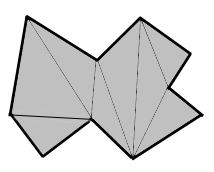
\includegraphics{rysunki/dual.png}
%     \caption{Wielokąt podzielony na trójkąty}
% \end{figure} 
% Z grafu dualnego usuwamy dowolny liść wraz z odpowiadającym mu trójkątem, kolorujemy wierzchołki wielokąta a następnie dodajemy trójkąt z powrotem nadając mu kolor inny niż sąsiadom.
% \begin{figure}[ht!]
%   \centering
%     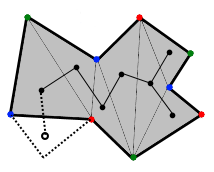
\includegraphics{rysunki/dual_kolor.png} 
%     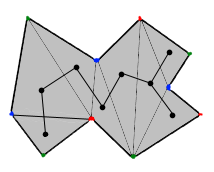
\includegraphics{rysunki/dual_caly_kolor.png}
%     \caption{Pokolorowany wielokąt wraz z grafem dualnym}
% \end{figure} 
% Strażników rozmieszczamy w tych wierzchołkach, których kolor jest najrzadziej używanym.
% \newpage\indent Ograniczenie g(n)$\le$$\floor{\frac{n}{3}}$ nie oznacza, że wystarczy rozmieścić strażnika w co trzecim wierzchołku. 
% \begin{figure}[ht!]
%   \centering
%   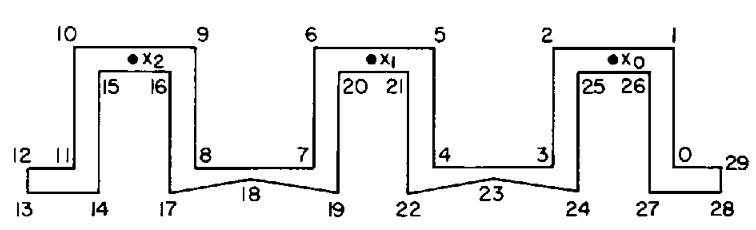
\includegraphics{rysunki/co_trzeci.png}
%   \caption{Punkt x jest niestrzeżony, przy rozmieszczeniu strażników w co trzecim wierzchołku.}
% \end{figure} 

% \subsection{Wielokąty z dziurami}
% Ciekawym rozwinięciem klasycznego zagadnienia galerii sztuki jest wprowadzenie dziur do wnętrza wielokąta.

% \begin{Definicja}\label{def wielokat z dziurami}
%   \textnormal{Wielokątem z dziurami} nazywamy wielokąt P, który mieści w sobie wiele innych wielokątów $H_1$, \ldots, $H_n$ nazywanych dziurami.
% \end{Definicja}
% Dodatkowo, żaden wielokąt nie może przecinać zarówno krawędzi wielokąta \textit{P} jak i innych wielokątów wewnętrznych $H_i$.

% \indent Podobnie jak w przypadku standardowych wielokątów, również dla wariantu z dziurami, aby obliczyć potrzebną ilość strażników, wykorzystamy triangulację.

% \begin{Lemat}
%   Każdy wielokąt P z dziurami, można podzielić na trójkaty.
% \end{Lemat}

% \begin{Lemat}\label{t trójkątów triangulacja}
%   Każdy wielokąt P o \textnormal{h} dziurach oraz \textnormal{n} krawędziach poddany triangulacji, dzieli się na \textit{t = n + 2h - 2} trójkątów.
% \end{Lemat}

% W dowodzie skorzystam z twierdzenia Eulera.
% \begin{Twierdzenie}\label{tw eulera}
%   Niech G będzie spójnym grafem planarnym o N wierzchołkach, M krawędziach oraz F ścianach. Wtedy N - M + F = 2.
% \end{Twierdzenie}

% Korzystając z tw. Eulera \ref{tw eulera}, V = n wierzchołków, F = t + h + 1 ścian (po jednej na każdy trójkąt oraz dziurę i ścianę zewnętrzną) a E = $\frac{3t+n}{2}$ krawędzi (trzy krawędzie na każdy trójkąt plus krawędzie zewnętrzne liczone podwójnie).  Wtedy \textit{V - E + F = 2} a więc \textit{n - $\frac{3t+n}{2}$ + t + h + 1 - 2} z czego wynika, że \textit{t = n + 2h - 2}.
% % \indent Niech zęwnętrzna krawędź wielokąta \textit{P} posiada $n_0$ krawędzi oraz niech \textit{i-ta} dziura posiada $n_i$ krawędzi wtedy \textit{n = $n_0$ + $n_1$ + \ldots + $n_i$}. W takim wypadku suma wewnętrznych kątów zewnętrznej krawędzi wynosi ($n_0$ - 2)*180 stopni a suma kątów zewnętrznych jesst równa ($n_i$ + 2)*180.
% % \todo{rysunek bo niewiadomo o co chodzi}
% % Taki wynik można zapisać jako sumę:
% % \\\textit{180(($n_0$ - 2) + ($n_1$ + 2) + \ldots + ($n_k$ +2)) = 180t $\implies$ t = n + 2i - 2}.


% Wiedząc, na ile trójkątów został podzielony wielokąt \textit{P}, możemy przejść do twierdzenia określającego wymaganą ilość strażników.

% \begin{Twierdzenie}[O'Rourke 1982]
%   Dla wielokąta o n wierzchołkach oraz h dziurach $\floor{\frac{n+2h}{3}}$ = $\ceil{\frac{t}{3}}$ strażników kombinatorycznych jest wystarczających aby dominować każdą triangulację wielokąta.
% \end{Twierdzenie}

% \indent Główną ideą dowodu jest kolejne usuwanie dziur wielokąta, wzdłuż przekątnych dodanych podczas triangulacji, poprzez łączenie ich ze ścianą zewnętrzną. Każda z dziur posiada krawędź w grafie triangulacji T, która łączy ją z inną dziurą lub z zewnętrzną krawędzią wielokąta P. ,,Przecięcie'' wzdłuż takiej krawędzi połączy dziurę ze ścianą zewnętrzną lub scali dwie dziury w jedną. W każdym z tych przypadków, całkowita ilość dziur zmniejszy się o jeden. Trudność polega jedynie na wyborze krawędzi z T, które pozwolą uzyskać taki podział.

% \indent Niech T' będzie grafem dualny triangulacji \textit{T}. \textit{T'} jest grafem planarnym, co najwyżej trzeciego stopnia, posiadającym \textit{h} graniczących ze sobą scian \textit{$F_1$, \ldots, $F_h$}, po jednej na każdą dziurę wielokąta P. Niech $F_0$ będzie ścianą zewnętrzną. Wybieramy dowolną ścianę $F_i$, która posiada przynajmniej jedną wspólną krawędź \textit{e} ze ścianą $F_0$. Taka krawędź istnieje, ponieważ w grafie \textit{T} musi istnieć przekątna łącząca krawędź zewnętrzną wielokąta \textit{P} z dowolną dziurą - w grafie \textit{T'} jest to krawędź \textit{e}. Usunięcie krawędzi \textit{e} z \textit{T'} scala \textit{$F_i$} z $F_0$, bez rozspójniania grafu.

% \begin{figure}[h!]
%   \centering
%     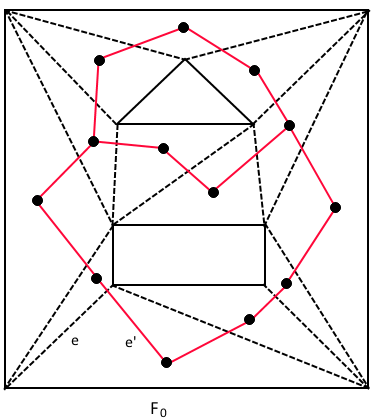
\includegraphics{rysunki/triangulacja_dziury.png}
%     \caption{Wielokąt z dziurami wraz z grafem dualnym. Krawędź \textit{e} odpowiada krawędzi \textit{e'} w grafie dualnym.}
%     \vspace{3in}
% \end{figure} 

% \indent Niech \textit{P'} będzie wielokątem uzyskanym według powyższej procedury. W takim wypadku \textit{P'} posiada \textit{n + 2h} krawędzi oraz \textit{t} trójkątów, ponieważ każde cięcie daje nam dwie dodatkowe krawędzie ale nie dodaje nowych trójkątów. Zgodnie z tw. Chv\'atala \textit{P'} potrzebuje $\floor{\frac{n+2h}{3}} = \ceil{\frac{t}{3}}$ strażników.

% \chapter{Strażnicy mobilni}
% \section{Strzeżenie wielokątów prostych przez strażników mobilnych}
% \subsection{Wprowadzenie}
% Jednym z najciekawszych wariantów problemu galerii sztuki, zaproponowanym przez Toussainta w 1981 roku, są strażnicy mobilni. Pomysł jest prosty -- zamiast rozmieszczać strażników w wierzchołkach wielokąta pozwalamy, aby dowolnie przemieszczali się w jego granicach.
% \begin{Definicja}
%   Niech \textit{s} będzie odcinkiem zawartym w wielokącie \textit{P}. Mówimy, że \textit{x} takiego, że \textit{x $\in$ P} jest strzeżony przez \textit{s}, jeżeli istnieje punkt \textit{y $\in$ s} taki, że odcinek \textit{xy $\subseteq$ P}.
%  \end{Definicja}

% \begin{figure}[ht!]
%   \centering
%     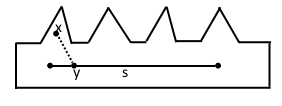
\includegraphics{rysunki/mobile_guard.png}
%     \caption{Strażnik poruszający się po prostej \textit{s} strzeże cały wielokąt}
% \end{figure} 
% 123
%  Zgodnie z powyższą definicją, \textit{x} jest strzeżone przez strażnika jeżeli jest widzialne z co najmniej jednego punktu odcinka po którym porusza się strażnik. Jest to tak zwana ,,słaba widoczność''. ,,Silna widoczność'' wymaga aby punkt \textit{x} był widoczny z każdego punktu na \textit{s}. 
% \\\indent Warto również zaznaczyć, że strażnicy mobilni są ,,silniejsi'' od strażników stacjonarnych. Średnio trzech strażników mobilnych jest w stanie pokryć taką samą przestrzeń jak czterech strażników stacjonarnych.
% \\\indent W tym rozdziale omówię dowód, że $\floor{\frac{n}{4}}$ strażników mobilnych jest czasami potrzebnych i zawsze wystarczających, aby strzec dowolny $n$-kąt.  

% \subsection{Ogólny dowód dla wielokątów}
% Na początku zdefiniujemy różne typy strażników geometrycznych. Na podstawie prostej, po której się poruszają dzielimy ich na 3 rodzaje:
% \begin{itemize}
% \item krawędziowy, który porusza się po krawędziach wielokąta łącznie z punktami końcowymi
% \item przekątniowy, który może się poruszać po odcinkach łączących krawędzie wielokąta
% \item odcinkowy, poruszający się po dowolnym odcinku zawierającym się we wnętrzu wielokąta
% \end{itemize}
% Każdy z powyższych strażników strzeże przestrzeń którą jest w stanie zobaczyć, poruszając się wzdłuż określonego odcinka.
% \\\indent Strażników rozmieszczonych w grafie \textit{T} wielokąta poddanemu triangulacji nazywamy strażnikami kombinatorycznymi. Strażnik wierzchołkowy to pojedynczy wierzchołek T, krawędziowy to para wierzchołków sąsiednich połączonych krawędzią grafu \textit{T}, która ma swój odpowiednik w wielokącie \textit{P} a ostatnim rodzajem jest strażnik przekątniowy, zdefiniowany przez parę dowolnych sąsiednich wierzchołków oraz krawędzie je łączące.
% Oczywiście, podobnie jak w przypadku strażników geometrycznych również od strażników kombinatorycznych wymagamy aby strzegli  daną przestrzeń. Odpowiednikiem strzeżenia dla tak zdefiniowanych strażników oraz grafu jest dominacja.
% \begin{Definicja}
% Zbiór strażników C = \{$g_1$,\ldots,$g_k$\} dominuje graf T jeżeli dla każdej ściany triangulacji T przynajmniej jeden z trzech wierzchołków należy do określonego $g_i$ $\in$ C.
% \end{Definicja}
% \begin{figure}[ht!]
%   \caption{Strażnicy $g_1$ oraz $g_2$ dominują graf T}
%   \centering
%     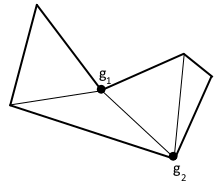
\includegraphics{rysunki/dominacja.png}
% \end{figure}
% Głównym założeniem jest, że $\frac{n}{4}$ strażników kombinatorycznych zawsze wystarcza a czasami jest wymaganych aby dominować graf triangulacji wielokąta z ilością wierzchołków \textit{n $\ge$ 4}.
% Z analogi strażników geometrycznych oraz kombinatorycznych wynika, że jeżeli graf triangulacji wielokąta jest dominowany przez \textit{k} wierzchołkowych strażników kombinatorycznych to może go strzec \textit{k} wierzchołkowych strażników geometrycznych. Powyższy wniosek pozwala nam stwierdzić, że dowód kombinatoryczny możemy rozszerzyć również na przypadek geometryczny.
% \\\indent Właściwy dowód przez indukcję przebiega podobnie jak dowód twierdzenia Chv\'atala. Jednak zanim przejdziemy do dowodu musimy  zdefiniować jeszcze jedną operację - ściąganie krawędzi.
% \begin{Definicja}
% W grafie G ściąganie krawędzi e łączącą wierzchołki u, v jest zamianą wierzchołków u, v na nowy, pojedynczy wierzchołek z którym incydentne są te krawędzie, które były incydentne z u oraz v. W rezultacie graf G' ma jedną krawędź mniej od G.
% \end{Definicja}
% \begin{figure}[ht!]
%   \caption{Graf G oraz G' po ściągnięciu krawędzi}
%   \centering
%     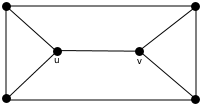
\includegraphics{rysunki/edge_contradiction1.png}
%     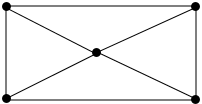
\includegraphics{rysunki/edge_contradiction2.png}
% \end{figure}
% \newpage
% Omówię teraz lematy, wraz z krótkimi dowodami, które zostaną wykorzystane w ostatecznym dowodzie.
% \begin{Lemat}
% Niech T będzie grafem triangulacji wielokąta P a T' grafem powstałym przez ściągnięcie jednej krawędzie T. Po takiej operacji T' jest grafem triangulacji jakiegoś wielokąta P'.
% \end{Lemat}
% Dowód polega na skonstruowaniu grafu z łukami odpowiadającego T' a następnie wyprostowaniu ich w celu uzyskania P'.
% \begin{Lemat}
% Załóżmy, że f(n) kombinatorycznych strażników zawsze wystarczy aby dominować dowolny graf triangulacji o n wierzchołkach. 
% Wtedy, jeżeli T jest danym grafem triangulacji wielokąta P ze strażnikiem wierzchołkowym umieszczonym w jednym z n wierzchołków grafu to dodatkowych f(n-1) strażników jest wystarczających aby dominować graf T.
% \end{Lemat}
% Innymi słowy, jedną z krawędzi możemy usunąć z obliczeń ilości strażników jeżeli istnieje strażnik umieszczony w dowolnym wierzchołku incydentnym z usuwaną krawędzią.
% \begin{Lemat}
% Każdy graf triangulacji pięciokąta foremnego jest dominowany przez pojedynczego kombinatorycznego strażnika przekątniowego z końcem w wybranym wierzchołku.
% \end{Lemat}
% Istnieje tylko 5 różnych triangulacji pięciokąta. Dla każdego z nich wystarczy jeden strażnik mobilny.
% \FloatBarrier 
% \begin{figure}[ht!]
%   \caption{Pięc triangulacji pięciokąta wraz ze strażnikami (przerywana linia ze strzałkami).}
%   \centering
%     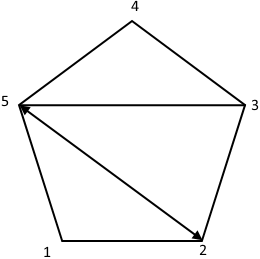
\includegraphics[width=4cm]{rysunki/pieciokat_triang_1.png}
%     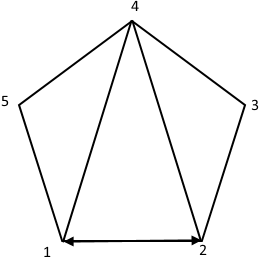
\includegraphics[width=4cm]{rysunki/pieciokat_triang_2.png}
%     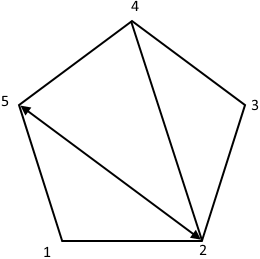
\includegraphics[width=4cm]{rysunki/pieciokat_triang_3.png}
%     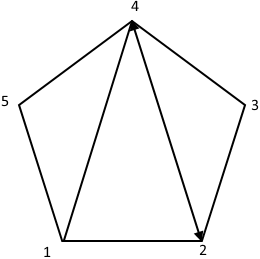
\includegraphics[width=4cm]{rysunki/pieciokat_triang_4.png}
%     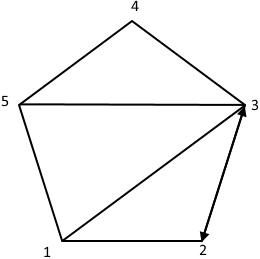
\includegraphics[width=4cm]{rysunki/pieciokat_triang_5.png}
% \end{figure}
% \FloatBarrier 
% \begin{Lemat}
% Każdy graf triangulacji siedmiokąta foremnego jest dominowany przez pojedynczego strażnika przekątniowego.
% \end{Lemat}
% Niech \textit{T} będzie grafem triangulacji siedmiokąta oraz niech \textit{d} będzie ustaloną przekątną wewnętrzną. Przekątna dzieli wielokąt w stosunku 2 krawędzie i pięciokąt lub 3 krawędzie i trapez.
% %\todo[inline]{Dlaczego 1+6 nie jest możliwe? 1+6 oznacza jedną krawędź i sześciokąt - niemożliwym jest poprowadzenie przekątnej która oddzieli jedną krawędź, minimum to 2}
% \begin{figure}[ht!]
%   \caption{Triangulacja siedmiokąta przy podziale 2+5 oraz 3+4}
%   \centering
% 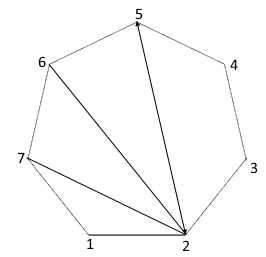
\includegraphics[width=5cm]{rysunki/siedmiokat_triang_1.png}
% 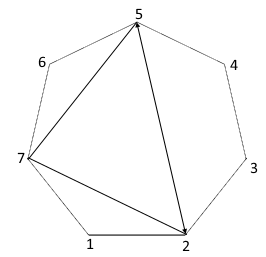
\includegraphics[width=5cm]{rysunki/siedmiokat_triang_2.png}
% \end{figure}
% \begin{Lemat}
% Każdy graf triangulacji dziewięciokąta jest dominowany przez dwóch strażników przekątniowych takich, że jeden koniec przekątnej jest incydentny z wybranym wierzchołkiem.
% \end{Lemat}
% Niech \textit{T} będzie grafem triangulacji dziewięciokąta foremnego, wybrany wierzchołek jest etykietowany numerem 1 a przekątna \textit{d} będzie dowolną przekątną wewnętrzną z końcem w wierzchołku 1. Taka przekątna dzieli krawędzie \textit{T} na 2 + 7, 3 + 6 lub 4 + 5.
% \begin{figure}[ht!]
%   \caption{Dziewięciokąt wraz z podziałami 2+7, 3+6 i 4+5}
%   \centering
% 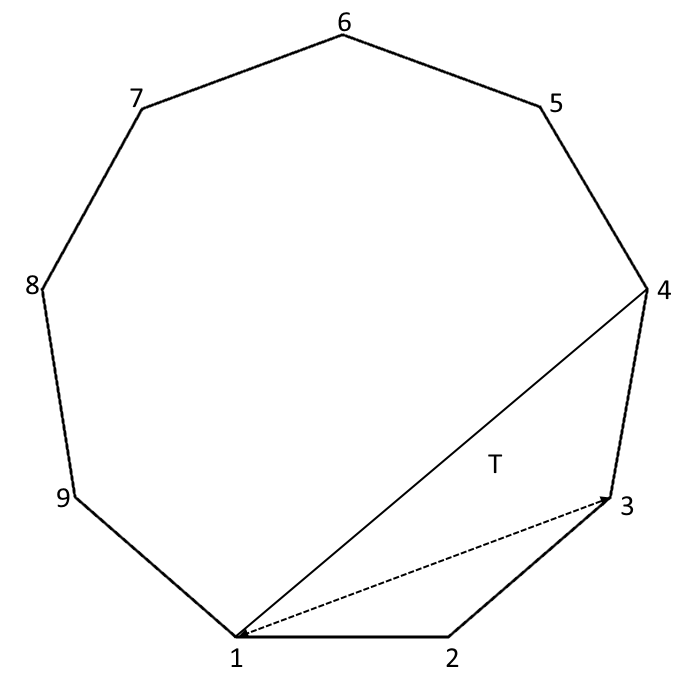
\includegraphics[width=6cm,height=6cm]{rysunki/dziewieciokat_triang_1.png}
% 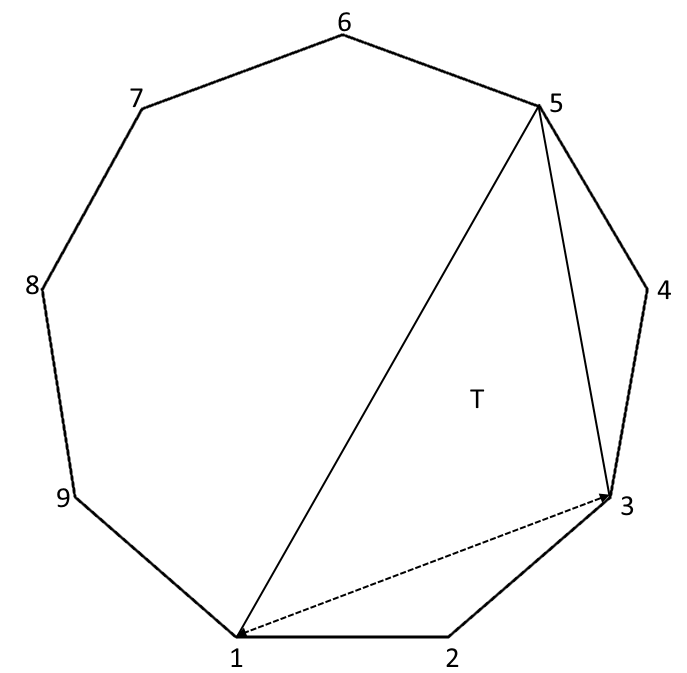
\includegraphics[width=6cm,height=6cm]{rysunki/dziewieciokat_triang_2.png}
% 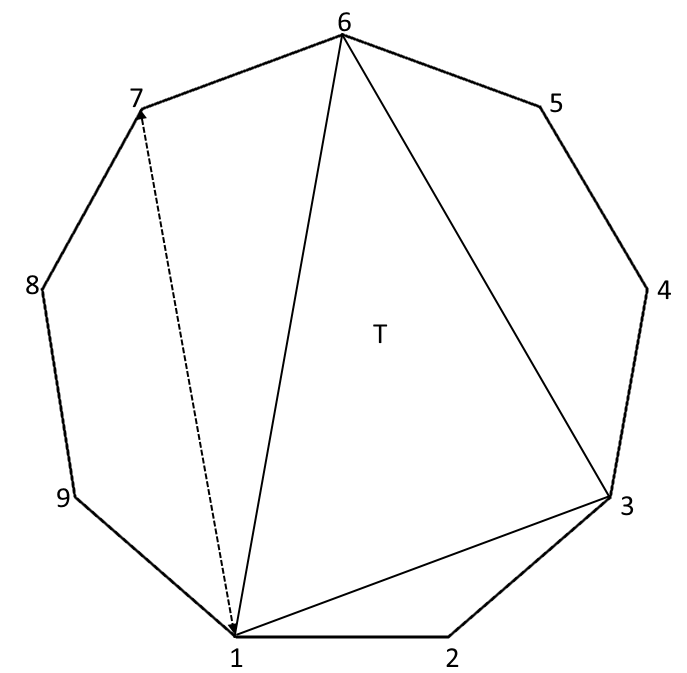
\includegraphics[width=6cm,height=6cm]{rysunki/dziewieciokat_triang_3.png}
% \end{figure}
% \\\indent Aby zakończyć dowód potrzebujemy jeszcze jednego podziału, który pozwoli nam wykorzystać indukcję dla \textit{n $\ge$ 10} wierzchołków. W tym celu użyjemy następującego lematu.
% \\\\\begin{Lemat}
% Niech \textit{P} będzie wielokątem o n $\ge$ 10 wierzchołkach oraz T będzie jego grafem triangulacji. Istnieje przekątna d w grafie T która dzieli go na dwie części, z których jedna zawiera k = 5,6,7 lub 8 łuków odpowiadających krawędziom P.
% \end{Lemat}
% Niech \textit{d} będzie przekątną grafu \textit{T} dzielącą minimalną ilość krawędzie wielokąta, która wynosi co najmniej 5. Niech \textit{k $\ge$ 5} będzie minimalną ilością krawędzi, wierzchołki posiadają etykiety 0,1,\ldots,n-1 a przekątna \textit{d} prowadzi prowadzi od wierzchołka 0 do \textit{k}. Przekątna \textit{d} jest podstawą trójkąta \textit{T}, którego szczyt znajduje sie w punkcie \textit{t}, \textit{0 $\le$ t $\le$ k}. Jako, że \textit{k} jest najmniejsze z możliwych, \textit{t $\le$ 4} i \textit{k - t $\le$ 4}, suma obu nierówności daje nam \textit{k $\le$ 8}.
% Biorąc pod uwagę wcześniej przedstawione lematy, dowód indukcyjny jest analizą wszystkich przypadków.
% \begin{Definicja}[O'Rourke, 1983]
% Każdy graf triangulacji T wielokąta o przynajmniej n $\ge$ 4 wierzchołkach jest dominowany przez $\floor{\frac{n}{4}}$ kombinatorycznych strażników przekątniowych.
% \end{Definicja}
% Lemat 4, 5 oraz 6 opisują problem dla \textit{5 $\le$ n $\le$ 9}. Załózmy, że \textit{n $\ge$ 10} oraz, że dowód działa dla każdego \textit{n$^\prime$ $<$ n}. Lemat 7 gwarantuje, że istnieje przekątna, która dzieli \textit{T} na dwa grafy \textit{$T_1$} oraz \textit{$T_2$}, gdzie \textit{$T_1$} zawiera \textit{k} krawędzi T dla \textit{4 $\le$ k $\le$ 8}. Rozpatrzymy teraz każdą wartość \textit{k}.
% \begin{enumerate}
% \item (k = 5 lub 6). $T_1$ ma \textit{k+1 $\le$ 7} krawędzi łącznie z \textit{d} oraz tworzy siedmiokąt. Zgodnie z lematem 5 $T_1$ jest dominowany przez pojedynczego strażnika. $T_2$ ma \textit{n - k + 1 $\le$ n - 5 + 1 = n - 4} krawędzi łącznie z d i zgodnie z założeniem indukcyjnym jest dominownay przez $\floor{\frac{n-4}{4}}$ = $\floor{\frac{n}{4}}$ - 1 strażników przekątniowych. W sumie dla $T_1$ oraz $T_2$ daje to $\floor{\frac{n}{4}}$ strażników przekątniowych.
% \item (k = 7). Jakakolwiek z przekątnych (0,6), (0,5), (1,7) lub (2,7) prowadziłaby do \textit{k $<$ 4}. W rezultacie trójkąt \textit{T} w $T_1$ musi być rozpięty przez (0,3,7) lub (0,4,7). Są to przypadki analogiczne więc załóżmy, że \textit{T} jest trójkątem o wierzchołkach (0,3,7). Czworokąt (0,1,2,3) ma dwie różne triangulacje, które rozpatrzymy osobno.
% \begin{enumerate}
% \item (punkty 1,3) Pięciokąt (3,4,5,6,7) dominuje jeden strażnik z końcem w punkcie 3, zgodnie z lematem 4. Ów strażnik dominuje cały graf \textit{$T_1$}. Skoro \textit{$T_2$} ma \textit{n - 7 + 1 = n - 6} krawędzi jest dominowany przez $\floor{\frac{n-6}{4}}$ $\ge$ $\floor{\frac{n}{4}}$ - 1 strażników przekątniowych zgodnie z tezą indukcyjną.
% \begin{figure}[ht!]
%   \centering
%  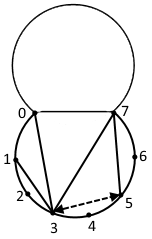
\includegraphics{rysunki/7a.png}
%   \caption{Graf triangulacji wraz ze strażnikiem (linia przerywana) dominującym graf}
% \end{figure}
% \item (punkty 0,2) Stwórzmy graf $T_0$ przez połączenie dwóch trójkątów \textit{T = (0,3,7)} i \textit{T' = (0,2,3)} .
% $T_0$ posiada \textit{n - 7 + 3 = n - 4} krawędzie więc jest dominowany przez $\floor{\frac{n-4}{4}}$ = $\floor{\frac{n}{4}}$ - 1 strażników przekątniowych zgodnie z tezą indukcyjną. W takim przypadku przynajmniej jeden z wierzchołków \textit{T' = (0,2,3)} musi być punktem końcowym strażnika przekątniowego. Daje nam to trzy przypadki:
% \begin{enumerate}
% \item Jeżeli 0 jest końcem przekątnej to do $T_0$ możemy dołączyć (0,1,2) bez potrzeby dodawania kolejnych strażników.
% \item Jeżeli 2 jest końcem przekątnej to możemy dołączyć (0,1,2) do $T_0$
% \item Jeżeli 3 jest końcem przekątnej, wtedy mamy trzy kolejne możliwości rozmieszczenia drugiego końca. Przypadki kiedy drugi koniec jest w 0 lub 2 rozpatrzyliśmy powyżej. Jeżeli jest on w 7 to zamieniamy przekątną strażnika z (3,7) na (0,7). Każdy trójkąt wciąż pozostaje zdominowany a $T_0$ ponownie możemy rozszerzyć o (0,1,2).
% \end{enumerate}
% \end{enumerate}
% Po rozpatrzeniu wszystkich przypadków możemy stwierdzić, że pięciokąt (3,4,5,6,7) jest domiowany przez $\floor{\frac{n}{4}}$ -1 strażników przekątniowych
% \begin{figure}[ht!]
%   \centering
%  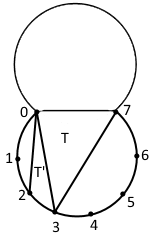
\includegraphics{rysunki/7b.png}
%   \caption{Graf triangulacji wraz ze strażnikiem dominującym graf}
% \end{figure}
% \item (k = 8) $T_1$ ma \textit{k + 1 = 9} krawędzi a więc zgodnie z lematem 6 jest dominowany przez dwóch strażników przekątniowych. Jedna z takich przekątnych kończy się w wierzchołku 0. $T_2$ ma \textit{n - k + 1 = n - 7} krawędzi. Według lematu 3 jeden strażnik w wierzchołku 0 pozwala na dominację pozostałej części $T_2$ przez \textit{f(n - 7 - 1) = f(n - 8)} strażników przekątniowych, gdzie \textit{f(n')} określa ilość strażników przekątniowych zawsze potrzebnych aby dominowac graf triangulacji o \textit{n'} wierzchołkach. Zgodnie z tezą indukcyjną \textit{f(n') = $\floor{\frac{n'}{4}}$} a  więc \textit{$\floor{\frac{n-8}{4}}$ = $\floor{\frac{n}{4}}$ - 2 } strażników przekątniowych dominuje $T_2$. Wspólnie z dwoma strażnikami umieszczonymi w $T_1$ caly graf \textit{T} jest dominowany przez $\floor{\frac{n}{4}}$ strażników przekątniowych.
% \begin{figure}[ht!]
%   \centering
%  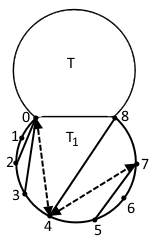
\includegraphics{rysunki/8.png}
%   \caption{Graf triangulacji oraz strażnicy dominujący graf}
% \end{figure}
% \end{enumerate}
% \FloatBarrier
% \begin{Twierdzenie}
% Każdy wielokąt P o n $\ge$ 4 krawędziach jest strzeżony przez $\floor{\frac{n}{4}}$ geometrycznych strazników przekątniowych lub linowych.
% \end{Twierdzenie}
% Ilość strażników przekątniowych wynika z wcześniejszego dowodu. Jako, że strażnicy przekątniowi są szczególnym przypadkiem strażników liniowych, taka sama ilość silniejszych strażników liniowych jest również wystarczająca.

% \chapter{Strzeżenie zbioru odcinków}
% \section{Strzeżenie zbioru odcinków}
% \subsection{Wprowadzenie}
% Ten wariant zagadnienia galerii sztuki wymaga, aby strzeżony odcinek był widoczny przez strażnika przynajmniej w jednym punkcie. 
% \begin{Definicja}
% Niech F = \{$S_1$,\ldots,$S_n$\} będzie zbiorem \textit{n} prostych odcinków na płaszczyźnie. Zbiór punktów Q = \{$p_1$,\ldots,$p_k$\} strzeże F, jeżeli każdy element $S_i$ ze zbioru F zawiera punkt, który jest widziany przez przynajmniej jeden punkt $p_j$ należący do Q.
% \end{Definicja}
% Tak zdefiniowany problem możemy zobrazować przez strażników, którzy strzegą obrazu, jeżeli widzą przynajmniej jeden jego fragment. W takim przypadku nie można zdjąć obrazu ze ściany bez zaalarmowania strażnika.
% \begin{figure}[ht!]
%  \centering
%   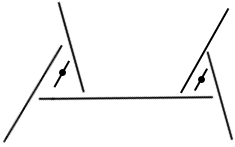
\includegraphics{rysunki/rozlaczny_dwoch_straznikow.png}
%   \caption{Zbiór odcinków rozłącznych wymagający dwóch strażników}
% \end{figure} 

% \begin{Twierdzenie}\label{straznicy strzezenie}
% Dowolny zbiór n odcinków prostych, jest zawsze strzeżony przez $\ceil{\frac{n}{2}}$ punktów a czasami wystarczających jest $\floor{\frac{2n-3}{5}}$ strażników.
% \end{Twierdzenie}

% \subsection{Ograniczenie górne}
% Aby udowodnić tw. \ref{straznicy strzezenie} na początku wykażemy, że dla każdej rodziny odcinków \textit{F}, których jest parzysta liczba \textit{n}, graf G(F) ma idealne skojarzenie.

% Rozpatrzmy teraz zbiór F = \{$S_1$,\ldots,$S_n$\} rozłącznych odcinków prostych na płaszczyźnie oraz graf G(F) zawierający \textit{n} odcinków $v_1$,\ldots,$v_n$ takich, że $v_i$ jest sąsiedni z $v_j$ wtedy i tylko wtedy, jeżeli istnieje punkt \textit{x} na płaszczyźnie, który widzi przynajmniej jeden punkt na odcinku $S_j$ i $S_i$ tzn. \textit{x} strzeże oba odcinki.

% \begin{figure}[ht!]\label{zbior odcinkow rozlacznych}
%  \centering
%   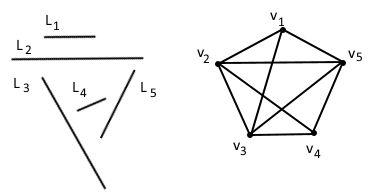
\includegraphics{rysunki/g_f.png}
%   \caption{Zbiór odcinków rozłącznych F oraz odpowiadający mu graf G(F)}
% \end{figure} 

% \begin{Lemat}\label{podgraf indukowany}
% Niech Q będzie dowolnym wielokątem prostym a F = \{$S_1$,\ldots,$S_n$\} rodziną n rozłącznych odcinków oraz niech H będzie podzbiorem elementów F, takich które przecinają wielokąt Q. Podgraf grafu G(F) indukowany przez wierzchołki G(F) reprezentujący elementy ze zbioru H jest spójny.
% \end{Lemat}
% \begin{figure}[ht!]
%  \centering
%   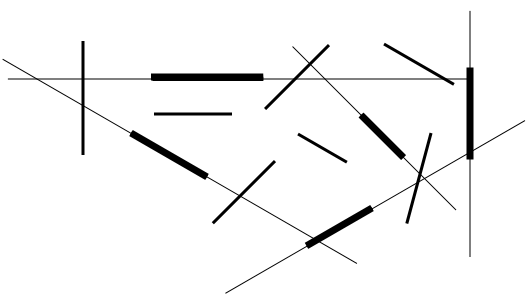
\includegraphics[height=3cm]{rysunki/podzial_h.png}
%   \caption{Podział zbioru F. Pogrubione elementy należą do zbioru H}
% \end{figure} 
% Niech \textit{F} = \{$S_1$,\ldots,$S_n$\} będzie zbiorem \textit{n} rozłącznych odcinków a \textit{G(F)} odpowiadającym mu grafem. Zakładamy, że \textit{n} jest parzyste, w przeciwnym wypadku należy dodać jeden odcinek do zbioru \textit{F}. Pokażemy teraz, że \textit{G(F)} spełnia twierdzenie Tutte'a a więc ma idealne skojarzenie.
% \\\indent Rozważmy dowolny podzbiór \textit{H} zbioru \textit{F} oraz niech \textit{S} będzie zbiorem wierzchołków grafu \textit{G(F)}, reprezentującego elementy \textit{H}. Pokażemy, że ilość spójnych części grafu \textit{G(F) - S} wynosi, co najwyżej |\textit{S}| = |\textit{H}|.
% \\\indent Na początku należy usunąć z płaszczyzny wszystkie odcinki, które nie należą do \textit{H}. Następnie, jeden po drugim przedłużamy elementy \textit{H} dopóki nie przetną innego elementu \textit{F}, wcześniej przedłużonego odcinka lub nie staną się prostymi bądź półprostymi. Niech $\pi$ oznacza płaszczyznę indukowaną przez przedłużone elementy zbioru \textit{H}. Łatwo zauważyć, że $\pi$ zawiera dokładnie |\textit{H}| + 1 ścian. Na końcu należy usunąć elementy \textit{F}, które nie należą do \textit{H}.
% \\\indent Zgodnie z lematem \ref{podgraf indukowany}, ilość elementów grafu \textit{G(F) - S} jest co najwyżej równa ilości ścian płaszczyzny $\pi$ czyli |\textit{H}| + 1. Możemy prosto sprawdzić, że występują przynajmniej dwie sąsiednie ściany z $\pi$ takie, że odcinki które je przecinają należą do tego samego elementu w grafie \textit{G(F) - S}. Stąd wniosek, że liczba elementów zbioru \textit{G(F) - S} wynosi co najwyżej |\textit{S}|, co implikuje, że \textit{G(F)} ma doskonałe skojarzenie \textit{M}. Na tej podstawie możemy stwierdzić, że wystarczy co najwyżej $\ceil{\frac{n}{2}}$ punktów aby strzec \textit{F} -- po jednym na każdy wierzchołek skojarzenia \textit{M}.
% \subsection{Ograniczenie dolne}
% \indent Aby uzyskać ograniczenie dolne, należy znaleźć \textit{n}-elementowy zbiór \textit{F}, który jest strzeżony przez $\floor{\frac{2n-3}{5}}$ strażników.
% \\\indent Niech \textit{H} będzie planarnym grafem kubicznym z trójkątną ścianą zewnętrzną, w której wszystkie wierzchołki, poza zewnętrznymi, spełniają założenie, że wektory wychodzące z wierzchołków wzdłuż krawędzi rozpinają płaszczyznę. \textit{H} posiada \textit{k} wierzchołków, wtedy ma $\frac{3k}{2}$ krawędzi.
% \\\indent Zamieniamy krawędzie zbioru \textit{H} na odcinki takie, że na każde \textit{k - 3} wewnętrzne wierzchołki przypadnie trójkątna ściana w której umieścimy mały odcinek.
% \begin{figure}[ht!]
%  \centering
%   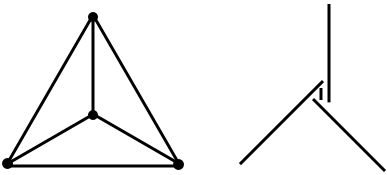
\includegraphics{rysunki/dolna_granica.png}
%   \caption{Przekształcenie grafu H.}
%   \label{fig:przeksztalcenie h}
% \end{figure} 
% Odrzucamy trzy krawędzie zewnętrznej ściany \textit{H} a następnie rozłączamy każdą krawędź w jej bliskim sąsiedztwie aby utworzyć zbiór \textit{n = ($\frac{3k}{n}$) - 3 + k  - 3} odcinków. Żadne dwa z \textit{k - 3} małych odcinków nie są widoczne z jednego punktu więc \textit{k - 3} punktów jest potrzebnych aby strzec taki zbiór. Możemy łatwo sprawdzić, że \textit{k - 3} punktów jest również wystarczające z czego wynika, ze \textit{k - 3 = $\floor{\frac{2n - 3}{5}}$} co kończy dowód twierdzenia \ref{straznicy strzezenie}.

% \section{Oświetlanie odcinków}\label{oświetlanie odcinków}
% \subsection{Wprowadzenie}
% Kolejną wariacją strzeżenie odcinków jest ich podświetlanie. Tym razem aby strzec odcinek wymagane jest jego podświetlenie. Należy zwrócić uwagę na fakt, że punkt na odcinku może zostać podświetlony również przez promień padający na niego z drugiej strony odcinka.

% \begin{Definicja}
%  Każdy zbiór F składający się z n rozłącznych odcinków możemy oświetlić przy użyciu co najwyżej $\ceil{\frac{2n}{3}}$ - 3 źródeł światła
% \end{Definicja}
% \subsection{Ograniczenie górne}
% \indent Niech \textit{F} = \{$L_1$, \ldots, $L_n$\} będzie zbiorem \textit{n} rozłącznych odcinków. Znajdźmy trójkąt \textit{T}, który zawiera wewnątrz wszystkie elementy ze zbioru \textit{F} oraz niech \textit{F'} będzie zbiorem zawierającym elementy \textit{F} oraz trzy odcinki $L_{n+1}$, $L_{n+2}$, $L_{n+3}$ uzyskane przez skrócenie boków trójkąta \textit{T} o $\epsilon$ $>$ 0
% Następnie należy stworzyć rodzinę zbiorów H = \{$S_1$,\ldots,$S_n$,$S_{n+1}$,$S_{n+2}$,$S_{n+3}$\} złożoną z \textit{n+3} ściśle wypukłych oraz wzajemnie rozłącznych zbiorów (zbiory mogą się stykać tylko w jednym punkcie -- na ich granicach) spełniającą następujące założenia:
% \begin{enumerate}
%   \item $L_i$ zawiera się w $S_i$, gdzie \textit{i} = 1,\ldots,n+3
%   \item Ilość punktów w których para elementów rodziny H styka się jest maksymalna
% \end{enumerate}
% \begin{figure}[ht!]
%  \centering
%   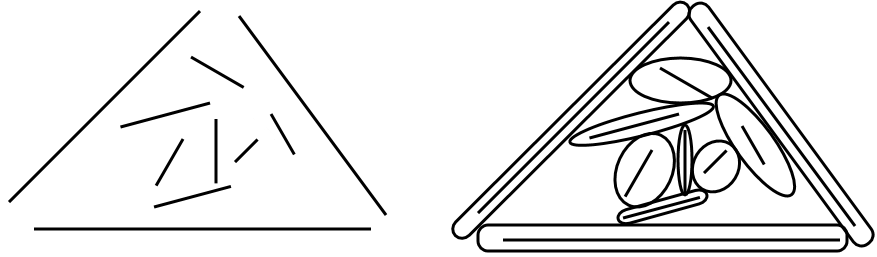
\includegraphics[height=5cm, width=13.5cm]{rysunki/podswietlenie.png}
%   \caption{Trójkąt ze zbioru F' i rodzina zbiorów H}
% \end{figure} 
% Możemy łatwo zauważyć, że elementy rodziny H są styczne z przynajmniej trzeba innymi elementami z tego zbioru. 
% \\Kolejnym krokiem jest stworzenie grafu \textit{G} poprzez zamianę każdego elementu zbioru \textit{H} na wierzchołek, przy założeniu, że dwa wierzchołki są sąsiednie jeżeli odpowiadające im zbiory są styczne.
% \begin{figure}[ht!]
%  \centering
%   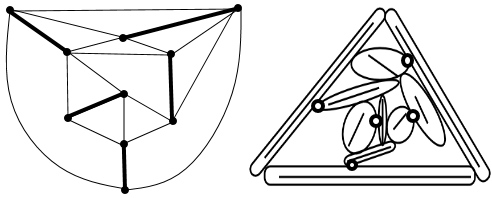
\includegraphics[height=4cm]{rysunki/skojarzenia_zrodla_swiatla.png}
%   \caption{Graf G oraz źródła światła}
% \end{figure}
% Tak stworzony graf jest planarny oraz 2-spójny. Jako, że każdy zbiór rodziny H jest styczny z co najmniej trzema innymi zbiorami, stopień każdego wierzchołka grafu \textit{G} wynosi co najmniej trzy. Zgodnie z twierdzeniem Nishizaki (1977) dla grafu \textit{G} istnieje co najmniej skojarzenie \textit{M} =  $\ceil{\frac{n+3+4}{3}} = \ceil{\frac{n+1}{3}}$  + 2. Dla każdej pary elementów $S_i$, $S_j$ skojarzonych w \textit{M} przez krawędź \textit{G}, należy umieścić źródło światła w punkcie ich przecięcia. W tak wyznaczonym punkcie światło będzie oświetlać odcinki $L_i$ oraz $L_j$ zawierające się, odpowiednio w $S_i$ oraz $S_j$. Jako, że skojarzenie \textit{M} ma przynajmniej $\ceil{\frac{n+1}{3}}$ + 2 elementów, 2($\ceil{\frac{n+1}{3}}$ + 2) elementy ze zbioru F wymagają $\ceil{\frac{n+1}{3}}$ + 2 świateł. W każdym z pozostałych elementów, które nie miały skojarzenia musimy rozmieścić po jednym źródle. W rezultacie uzyskujemy:
% ($\ceil{\frac{n+1}{3}}$ + 2) + ((n + 3) - 2($\ceil{\frac{n+1}{3}}$)) = n + 5 - $\ceil{\frac{n+1}{3}}$ $\le$ $\ceil{\frac{2n}{3}}$ + 3

% \subsection{Ograniczenie dolne}
% \indent Granica dolna nie jest precyzyjnie określona. Przykładem zbioru dla którego wystarczy $\floor{\frac{2n-3}{5}}$ źródeł światła jest np. rysunek \ref{fig:przeksztalcenie h} ze źródłem światła umieszczonym na wewnętrznym odcinku.

% \subsection{Luka między ograniczeniem górnym a dolnym}
% Z racji dużej nieścisłości pomiędzy ograniczeniem górnym a dolnym, znalezienie dokładnego wyniku wciąż jest problemem otwartym. Do tej pory nie udało się znaleźć dowodu chociażby na ograniczenie $\ceil{\frac{n}{2}}$ + c, gdzie \textit{c} jest stałą.

% \section{Ukrywanie się za ścianami}
% \subsection{Wprowadzenie}
% Po raz pierwszy problem ten przedstawili Hurtado, Serra oraz Urrutia (1996). Zdefiniowali oni problem w następujący sposób.

% \begin{Definicja}\label{ukrywanie definicja}
%  Rozpatrzmy zbiór rozłącznych odcinków F. Zbiór punktów P nazywamy ukrytym w stosunku do F, jeżeli dowolna linia łącząca dwa punkty ze zbioru P przecina element zbioru F.
% \end{Definicja}

% \begin{Definicja}\label{podciag rosnacy}
%   W każdym ciągu n liczb istnieje podciąg o długości co najmniej $\sqrt{n}$, rosnący lub malejący.
% \end{Definicja}

% Dla tak zdefiniowanego problemu, korzystając z twierdzenia Erdosa i Szekeresa, uzyskali oni dokładne ograniczenie przez $\sqrt{n}$.
% \begin{Twierdzenie}\label{moc zbioru ukrytego tw}
%   Dowolna rodzina n rozłącznych odcinków posiada zbiór punktów ukrytych o mocy co najmniej $\sqrt{n}$.
% \end{Twierdzenie}

% \subsection{Dowód twierdzenia \ref{moc zbioru ukrytego tw}}
% Rozpatrzmy zbiór \textit{F} = \{$L_1$,\ldots,$L_n$\} odcinków takich, że ich rzut na oś OX tworzy rozłączny zbiór. Przez $\alpha_i$ oznaczamy nachylenie $L_i$ dla \textit{i} = 1,\ldots,n w stosunku do osi OX.

% \begin{Lemat}\label{zbior ukryty}
%   Jeżeli $\alpha_1$ $<$ $\alpha_2$, \ldots, $<$ $\alpha_n$ to F posiada ukryty zbiór rozmiaru n.
% \end{Lemat}

% Dla każdego odcinka $L_i$ niech punkt $p_i$ będzie jego środkiem. Wybieramy punkt $q_i$, poniżej $p_i$, w odległości $\epsilon$ od $L_i$, \textit{i} = 1,\ldots,n. Następnie zakładamy, że jeżeli $\epsilon$ jest dostatecznie mały to $q_1$, \ldots, $q_n$ tworzy zbiór ukryty. Rozpatrzmy dwie liczby całkowite \textit{i} $<$ \textit{j} oraz odcinek $L_{ij}$ łączący $p_i$ z $p_j$. Jeżeli $\alpha_i$ jest mniejsze niż nachylenie $\alpha_{ij}$ odcinka $L_{ij}$, wtedy wybierając $\epsilon$ wystarczająco mały, gwarantujemy, że odcinek łączący $q_i$ z $q_j$ przecina $L_i$. Jeżeli $a_i$ jest większe lub równe $\alpha_{ij}$ to odcinek łączący $q_i$ z $q_j$ przetnie $L_j$. Obrazuje to rysunek \ref{fig:5 zbior ukryty}
% \begin{figure}[ht!]
%   \centering
%    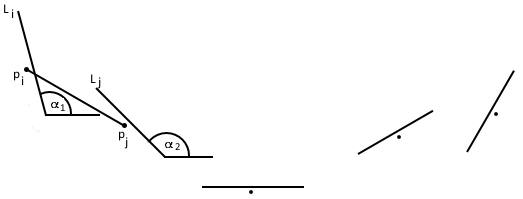
\includegraphics{rysunki/5_odcinkow_zbior_ukryty.png}
%    \caption{Zbiór 5 odcinków o rosnącym nachyleniu, który posiada zbiór ukryty o rozmiarze równym 5}
%    \label{fig:5 zbior ukryty}
% \end{figure}
% \\Przejdźmy teraz do właściwego dowodu twierdzenia \ref{moc zbioru ukrytego tw}.
% \\Rozpatrzmy rodzinę \textit{n} rozłącznych odcinków. Wybieramy punkt $p_i$ na każdym z odcinków $L_i$, w taki sposób aby współrzędne $x_1$,\ldots, $x_n$ dla $p_i$,\ldots,$p_n$ były różne. Możemy założyć, bez straty ogólności, że $x_1$ $<$ $x_2$ $<$ \ldots $<$ $x_n$. Następnie, dla każdego $L_i$ wybieramy odcinek $L'_i$ zawierający się w nim, ze środkiem w punkcie $p_i$ w taki sposób, że rzut na oś OX $L'_i$,\ldots,$L'_n$, tworzy zbiór rozłączny. Rozważmy teraz ciąg nachyleń $L'_1$, \ldots, $L'_n$. Zgodnie z def. \ref{podciag rosnacy} taki ciąg zawiera podciąg rosnący lub malejący o rozmiarze co najmniej $\sqrt{n}$, co biorąc pod uwagę lemat \ref{zbior ukryty}, kończy dowód.

% \chapter{K-nadajniki}
% \section{K-Nadajniki}
% \subsection{Wprowadzenie}
% Ilość sieci wifi cały czas rośnie, zarówno w naszych domach jak i w miejscach ogólnodostępnych. Fabila-Monroy, Aichholzer zainspirowani postępującą technologią przedstawili nowy problem, ściśle związany z teorią galerii sztuki. Opracowany przez nich wariant, nazywany ,,oświetleniem modemowym'', definiuje strażnika jako bezprzewodowy nadajnik o nieskończonym zasięgu oraz możliwości przebicia \textit{k} ,,ścian''. Ściany są zazwyczaj reprezentowane przez odcinki na płaszczyźnie. Problem zdefiniowali następująco:

% \textit{
%   Mając dany zbiór przeszkód na płaszczyźnie, liczbę naturalną k $>$ 0 oraz dany obszar, jak wiele  nadajników jest potrzebnych oraz koniecznych aby pokryć cały obszar?}  
% \\\indent Warto zauważyć, że zagadnienie dla 0-nadajników to klasyczny problem sztuki (strażnicy, którzy nie widzą przez ściany).
% \\W wypadku, gdy wymagamy strzeżenia całej płaszczyzny nadajnik możemy umieścić wewnątrz ściany, co pozwala nadawać po jej obu stronach.

% \section{Pokrycie płaszczyzny z przeszkodami}
% \subsection{Odcinki prostopadłe}
% W tym podrozdziale omówię wariant, w którym przeszkodami będzie zbiór \textit{n} rozłącznych odcinków prostopadłych a celem będzie pokrycie całej płaszczyzny. Czyżowicz i inni dowiedli, że $\ceil{\frac{n+1}{2}}$ 0-nadajników zawsze wystarcza a czasami jest koniecznych aby pokryć całą płaszczyznę na której znajduje się \textit{n} rozłącznych prostopadłych odcinków. Ballinger i inni rozszerzyli to ograniczenie dla k-najdaników.
% \begin{Definicja} \label{ograniczenie zbiór odcinków prostopadłych}
%   $\ceil{\frac{5n+6}{12}}$ 1-nadajników jest zawsze wystarczających a $\ceil{\frac{n+1}{4}}$ czasami koniecznych aby pokryć całą płaszczyznę z n rozłącznymi odcinkami prostopadłymi.
% \end{Definicja}
% \indent Łatwo ustalić dolną granicę ponieważ pojedynczy 1-nadajnik może pokryć co najwyżej cztery z \textit{n + 1} obszarów, z czego wynika, że potrzebujemy $\ceil{\frac{n+1}{4}}$ 1-nadajników dla \textit{n} lini równoległych.
% \begin{figure}[ht!]
%   \centering
%   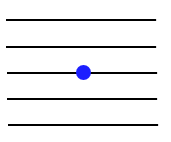
\includegraphics{rysunki/k_nadajniki_ogr_dolne.png}
%   \caption{1-nadajnik strzegący 4 obszarów}
%   \label{fig:ogr_dolne}
% \end{figure} 
% \\\indent Ograniczenie górne uzyskamy korzystając z następującego algorytmu:
% \begin{itemize}
%   \item ze zbioru wszystkich odcinków \textit{S} usuń odcinki niezależne
%   \item rozmieść 0-nadajniki
%   \item zwiększ zasięg przekaźników o jeden
% \end{itemize}

% W pierwszym kroku przedłużamy wszystkie odcinki, dopóki się nie przetną lub nie staną się półprostymi, jednocześnie dzieląc płaszczyznę na \textit{n + 1} ścian. Następnie tworzymy graf widzialności \textit{G(S)}, w którym każdy odcinek ze zbioru \textit{S} jest wierzchołkiem grafu. Krawędzie między wierzchołkami tworzymy jeżeli dwa odcinki \textit{s} i \textit{t} są słabo widzialne, tzn. istnieją punkty \textit{p} należący do odcinka \textit{s} oraz \textit{q} należący do odcinka \textit{t}, które połączone odcinkiem nie przecinają żadnego innego odcinka ze zbioru \textit{S}.

% \begin{Lemat}\label{0-1-nadajniki}
%   Jeżeli I jest niezależnym zbiorem w grafie G(S) a T jest zbiorem 0-nadajników, które pokrywają całą płaszczyznę S - I, to T jest również zbiorem 1-nadajników, które pokrywają całą płaszczyznę S.
% \end{Lemat}

% \indent Załóżmy, że 0-nadajnik w punkcie \textit{p} pokrywa punkt \textit{q} na płaszczyźnie \textit{S - I}. Odcinek \textit{pq} nie może przecinać dwóch lub więcej odcinków ze zbioru \textit{I}, ponieważ wtedy takie odcinki nie byłyby niezależne. Jednocześnie, odcinek \textit{pq} nie przecina żadnego odcinka ze zbioru \textit{S - I} a więc 1-nadajnik w punkcie \textit{p} pokrywa \textit{q} na płaszczyźnie \textit{S}.
% \\\indent Aby uzyskać największy możliwy zbiór niezależny w \textit{G(S)}, kolorujemy graf \textit{G(S)} a następnie wybierzemy najliczniejszą klasę kolorów. Zakładamy, ze ściany powstałe przez przedłużenie odcinków w zbiorze \textit{S} są prostokątne (w przeciwnym wypadku są trójkątne a więc 4-kolorowalne). 
% Tak powstały graf jest 1-planarny oraz 6-kolorowalny (Ringel, 1965).

% \begin{Definicja}
%   Grafem 1-planarnym nazywamy graf, którego każda z krawędzi może przeciąć inną krawędź co najwyżej raz.
% \end{Definicja}
% \begin{figure}[ht!]
%   \centering
%   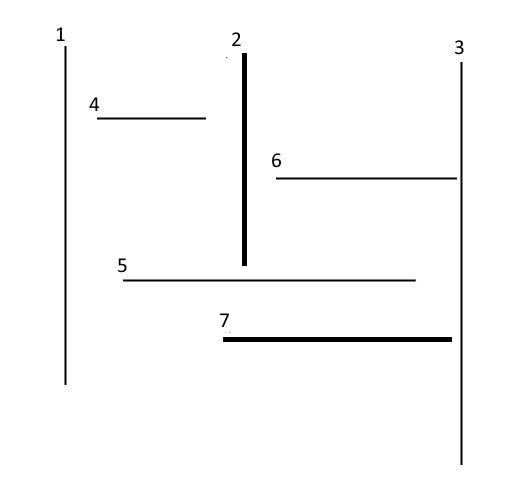
\includegraphics[width=6.5cm]{rysunki/zbior_odcinkow.png}
%   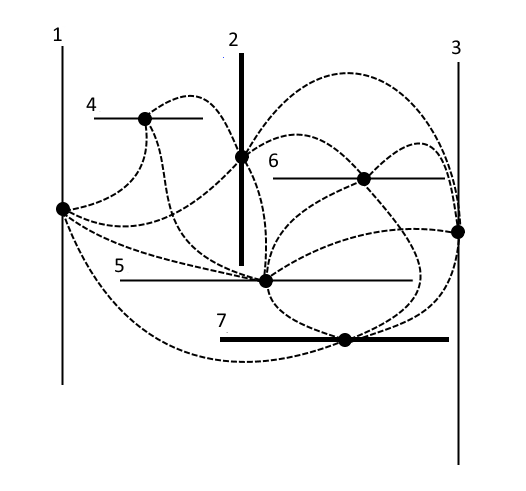
\includegraphics[width=6.5cm]{rysunki/graf_zbioru_odcinkow.png}
%   \caption{Zbiór odcinków S oraz graf G(S). Zbiór niezależny został pogrubiony.}
%   \label{fig:przedluzone odcinki}
% \end{figure} 

% \begin{Lemat}
%   Jeżeli S jest zbiorem przedłużonych odcinków prostopadłych to G(S) jest \textit{1-planarny}.
% \end{Lemat}
% \indent Jeżeli przedłużymy każdy odcinek zbioru \textit{S} to może on przecinać inny odcinek, co najwyżej w jednym punkcie, ponieważ odcinki są w stosunku do siebie równoległe, bądź prostopadłe. Tworząc graf \textit{G(S)} zamieniamy odcinki na wierzchołki, łącząc je krawędziami wtedy i tylko wtedy, gdy przecinają się lub są do siebie równoległe. Tak skonstruowany graf przedstawia rysunek \ref{fig:przedluzone odcinki}

% \indent Aby uzyskać ograniczenie górne kolorujemy graf \textit{G(S)} szcześcioma kolorami. Najliczniejsza klasa kolorów ma więc $\frac{n}{6}$ elementów oraz tworzy zbiór niezależny \textit{I}. Pozostały zbiór \textit{S - I} posiada $\frac{5n}{6}$ odcinków a więc zgodnie z rezultatem Czyżowicza potrzeba $\ceil{\frac{\frac{5n}{6} + 1}{2}}$ = $\ceil{\frac{5n+6}{12}}$ 0-nadajników, rozmieszczonych na odcinkach zbioru \textit{S - I} o tym samym kolorze. Następnie, zgodnie z lematem \ref{0-1-nadajniki} zwiększamy moc rozmieszczonych nadajników o jeden, co pozwala strzec całą płaszczyznę.
% \begin{figure}[ht!]
%   \centering
%   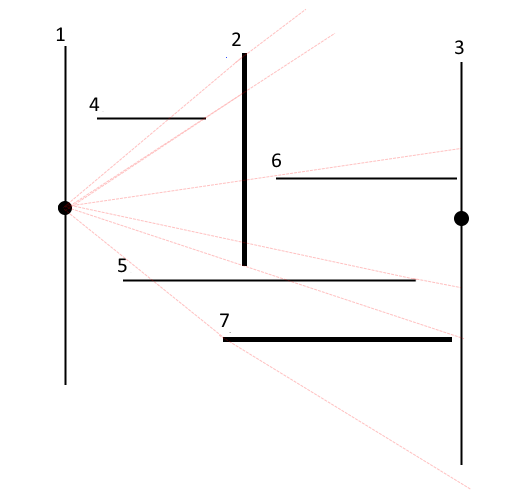
\includegraphics[width=6.5cm]{rysunki/pokrycie_nadajnikami.png}
%   \caption{Pokrycie płaszczyzny 1-nadajnikami.}
%   \label{fig:pokrycie plaszczyzny}
% \end{figure} 

% \section{Podział gilotynowy}
% Podział gilotynowy \textit{S} otrzymujemy przez dodanie kolekcji $s_1$,\ldots,$s_n$ odcinków prostych w taki sposób, że każdy dodany odcinek $s_i$ dzieli dowolną ścianę podzbioru $S_{i-1}$ na dwie nowe ściany tworząc nowy podział $S_i$. Ścianą $S_0$ nazywamy całą płaszczyznę.

% \begin{Twierdzenie}
%   Dowolny podział gilotynowy możemy pokryć $\frac{n+1}{2}$ 1-nadajnikami.
% \end{Twierdzenie}
% Dowód powyższego twierdzenia zaczniemy od lematu:
% \begin{Lemat}\label{sasiednie sciany strzega F}
%   Niech F będzie ścianą podziału gilotynowego S. Jeżeli każda inna ściana, która dzieli krawędź z F, posiada wewnątrz 1-nadajnik to taki zbiór nadajników pokrywa całe F.
% \end{Lemat}\label{nadajniki strzega f' i f}
% \indent Rozpatrzmy odcinek $s_i$, którego dodanie tworzy ścianę \textit{F}. Przed dodaniem odcinka $s_i$, podział $S_{i-1}$ zawierał jedną ścianę, która została podzielona na dwie części \textit{F} oraz \textit{F'} przez $s_i$. 
% % \begin{figure}[ht!]
% %   \centering
% %   \label{podzial F przez s_i}
% %   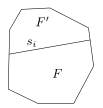
\includegraphics[width=9cm,height=6cm]{rysunki/podzial_F.png}
% %   \caption{Ściana F oraz F' po dodaniu odcinka $s_i$}
% % \end{figure} 


% W dalszym procesie ściana \textit{F} nie będzie już dzielona ale podzielimy ścianę \textit{F'} uzyskujac kolejne ściany $F'_1$, \ldots, $F'_k$, takie, że $F'_j$ $\subseteq$ F' oraz $F'_j$ dzieli część odcinka $s_i$ ze ścianą \textit{F} dla każdego \textit{j $\in$ \{1,\ldots,k\}}

% \begin{figure}[ht!]
%   \centering
%   \label{podzial F' na kolejne ściany}
%   \includegraphics[width=9cm,height=6cm]{rysunki/podzial_F'.png}
%   \caption{Kolejne podziały ściany F'}
% \end{figure} 
% Zgodnie z lematem \ref{nadajniki strzega f' i f} 1-nadajniki umieszczone wewnątrz ścian \textit{$F'_1$, \ldots, $F'_k$} strzegą wnętrza \textit{F}. 
% \\Aby to udowodnić, tymczasowo usuniemy odcinek $s_i$. W ten sposób uzyskamy podział \textit{S'}, przedłużając odcinki, którymi wcześniej dokonaliśmy podziału ściany \textit{F'}.

% \begin{figure}[ht!]
%   \centering
%   \label{podzial po usunieciu si}
%   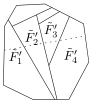
\includegraphics[width=9cm,height=6cm]{rysunki/usuniete_si.png}
%   \caption{Podział płaszczyzny po usunięciu odcinka $s_i$}
% \end{figure} 

% Po tej operacji, każda ze ścian \textit{$F'_j$} w \textit{S} powiększa się w \textit{S'} a dodatkowe części ścian sumują się do \textit{F}. Widzimy, ze każdy z 1-nadajników rozmieszczonych wewnątrz ścian \textit{$F'_j$} pokrywa przynajmniej \textit{$F'_j$} a więc razem nadajniki \textit{$F'_1$,\ldots,$F'_k$} strzegą ściany \textit{F}.

% \begin{Twierdzenie}
%   Dowolny podział gilotynowy strzeże co najwyżej $\frac{n+1}{2}$ 1-nadajników.
% \end{Twierdzenie}
% \indent Rozpatrzmy graf dualny \textit{T} podziału. \textit{T} jest triangulacją o \textit{n + 1} krawędziach. Niech \textit{M} będzie maksymalnym skojarzeniem w grafie \textit{T}. Każda nieskojarzona krawędź jest incydentna tylko z krawędziami skojarzonymi ( w przeciwnym przypadku skojarzenie nie byłoby maksymalne). Niech \textit{G} będzie zbiorem 1-nadajników, uzyskanych przez rozmieszczenie ich w pierwszej skojarzonej krawędzi \textit{e $\in$ M}. W takim wypadku |\textit{G}| = |\textit{M}| $\le \frac{n+1}{2}$. Dla każdej ściany \textit{F} z \textit{S}, \textit{F} albo zawiera 1-nadajnik w \textit{G} albo wszystkie sąsiednie ściany, które dzielą krawędź z \textit{F} zawierają 1-nadajnik w \textit{G}. W pierwszym przypadku \textit{F} jest oczywiście strzeżona. Natomiast w drugim przypadku, zgodnie z lematem \ref{sasiednie sciany strzega F}, ściana \textit{F} również jest strzeżona. Dlatego \textit{G} jest zbiorem 1-nadajników, które strzegą wszystkich ścian \textit{F} o mocy co najwyżej $\frac{n+1}{2}$
% \begin{figure}[ht!]
%   \centering
%   \label{pokrycie f}
%   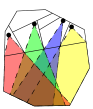
\includegraphics[width=9cm,height=6cm]{rysunki/pokrycie_f.png}
%   \caption{Nadajniki każdej ze ścian strzegące całą ścianę F}
%   \vspace{6in}
% \end{figure} 

% \chapter{Strażnicy na siatkach}
% \section{Siatki 2D}
% W 1986 roku Simeon Ntafos przedstawił koncept strażników strzegących specjalnej klasy wielokątów - siatek.
% Przez siatkę \textit{P} rozumiemy połączony zbiór poziomych oraz pionowych odcinków prostych. Możemy na nią spojrzeć jak na wielokąt prostokątny z dziurami, który składa się z bardzo cienkich korytarzy.
%  \begin{figure}[ht!]
%    \centering
%    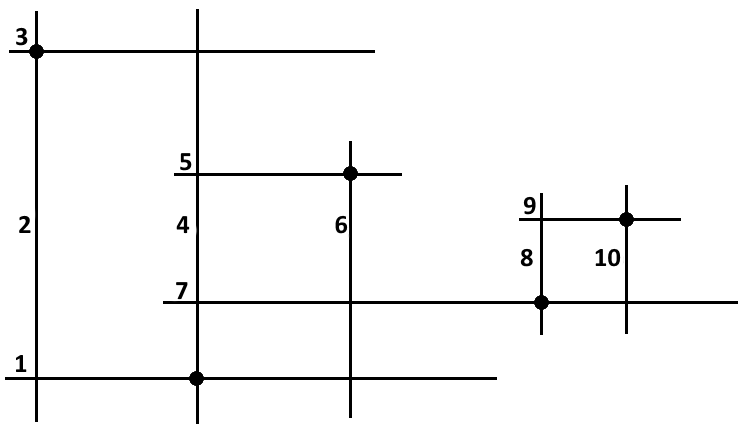
\includegraphics[width=14cm,height=6cm]{rysunki/przykladowa_siatka.png}
%    \caption{Siatka strzeżona przez 6 strażników}
%  \end{figure} 
% Widzialnością w siatce nazywamy sytuację, w której strażnik będący w punkcie \textit{x} widzi punkt \textit{y} jeżeli odcinek \textit{xy} należy do zbioru P (czyli jest korytarzem siatki).

% \begin{Twierdzenie}[Ntafos 1985]
% 	Minimalna ilość strażników potrzebna aby \textnormal{strzec siatkę} o \textnormal{n} odcinkach wymaga \textnormal{n - m} strażników, gdzie \textnormal{m} to moc doskonałego skojarzenie w grafie przecięć, które można znaleźć w czasie $\theta(n^{2.5})$
% \end{Twierdzenie}
% Ntafos zaproponował elegancki algorytm aby znaleźć minimalną ilość strażników potrzebną do strzeżenia siatki.
% \\\textbf{Dowód.}
% Aby strzec całej siatki, przynajmniej jeden strażnik musi znajdować się w każdym korytarzu. Niech \textit{G} będzie grafem przecięć siatki. Każdy wierzchołek z grafu \textit{G} odpowiada odcinkowi a dwa wierzchołki są połączone krawędzią wtedy i tylko wtedy, jeżeli odpowiadające im odcinki przecinają się.
%  \begin{figure}[ht!]
%    \centering
%    \label{fig:graf przeciec}
%    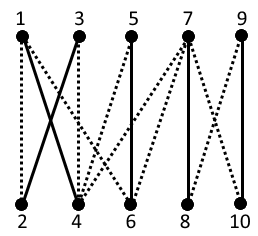
\includegraphics{rysunki/graf_skojarzen.png}
%    \caption{Graf przecięć siatki. Skojarzenia oznaczono linią ciągłą.}
%    \todo[inline]{Do poprawki rysunek}
%  \end{figure} 
%  \\Skojarzeniem w grafie \textit{G} nazywamy zbiór krawędzi \textit{M} takich, że każda krawędź z \textit{G} jest incydentna co najwyżej z jedną krawędzią z \textit{M}. Skojarzeniem doskonałym nazywamy takie skojarzenie, które ma maksymalną moc. W grafie przecięć \ref{fig:graf przeciec} skojarzenie to nic innego jak zbiór wszystkich przecięć korytarzy pionowych z poziomymi. Doskonałe skojarzenie dla dowolnego grafu o \textit{V} wierzchołkach można znaleźć w czasie O($V^{2.5}$) (Even 1979). Jako, że graf \textit{G} jest dwudzielny ponieważ przecięcia występują tylko pomiędzy korytarzamia pionowymi i poziomymi problem znalezienia maksymalnego skojarzenia sprowadza się do problemu kojarzenia małżeństw, który da się rozwiązać w czasie O($V^{1/2}$E), gdzie \textit{V} to ilość wierzchołków a \textit{E} ilość krawędzi w grafie dwudzielnym (Even 1979). Dla siatki o \textit{n} odcinkach \textit{V = n} a maksymalna ilość krawędzi to \textit{E = O($n^2$)} więc w najgorszym przypadku maksymalne skojarzenie znajdziemy w czasie O($n^{2.5}$).
%  \\\indent Aby strzec siatkę w całości, każdy odcinek wymaga strażnika a więc rozmieszczenie ich na przecięciach korytarzy pozwala strzec co najwyżej dwa odcinki. Stąd uzyskujemy minimalną ilość strażników wynoszącą $\ceil{\frac{n}{2}}$ dla siatki o \textit{n} odcinkach. Jeżeli graf posiada doskonałe skojarzenie o rozmiarze $\ceil{\frac{n}{2}}$ wtedy taka sama ilość strażników jest wystarczająca. Należy ich rozmieścić w każdym przecięciu korytarzy odpowiadającemu skojarzeniu w grafie. Jeżeli skojarzenie ma moc \textit{m}, wtedy rozmieszczenie w odpowiadającym im przecięciach strzeże \textit{2m} odcinków. W każdym z pozostałych \textit{n - 2m} odcinków musi zostać umieszczony jeden strażnik, co w sumie daje nam \textit{m + n - 2m = n - m} strazników. Jest to jednocześnie dolne ograczenie: jeżeli mniej niż \textit{n - m} strażników wystarcza, wtedy ponad \textit{m} strażników musi kryć dwa odcinki a to daje nam skojarzenie o rozmiarze większym niż \textit{m}, co nie jest możliwe.

%  \section{Siatki 3D}
%  	Ntafos przedstawił również zagadnienie strzeżenia siatki w trzech wymiarach, który to problem jest NP-zupełny. Dowód uzyskamy przez redukcję problemu pokrycia wierzchołkowego grafu co najwyżej trzeciego stopnia, który należy do klasy NPC (Garey i Johnson 1979).
% \begin{Definicja}
% 	Pokryciem wierzchołkowym grafu \textnormal{G = (V,E)} nazywamy podzbiór \textnormal{$V_0$ $\subseteq$ V} takich wierzchołków grafu, że każda krawędź z \textnormal{G} jest incydentna z przynajmniej jednym wierzchołkiem $V_0$.
% \end{Definicja}
% Naszym celem jest stworzenie trójwymiarowej siatki \textit{P}, którą możemy pokryć co najwyżej \textit{g} strażnikami wtedy i tylko wtedy jeżeli istnieje pokrycie wierzchołkowe \textit{G} przez co najwyżej \textit{K} wierzchołków.
% W tym celu etykietujemy wszystkie wierzchołki grafu \textit{G} kolejnymi liczbami 1,2,\ldots,n = |V|. Następnie, przypisujemy wierzchołki punktom siatki wzdłuż prostej poprowadzonej pomiędzy punktami (0,0,0) i (1,1,1) tak, aby każdy wierzchołek \textit{i} otrzymał punkt siatki \textit{$v_i$ = (3i, 3i, 3i)}. Krawędzie \textit{G} reprezentowane są przez linie łączące węzły siatki. Jako, że każdy wierzchołek grafu \textit{G} jest stopnia co najwyżej trzeciego, każdej incydentnej krawędzi możemy przypisać jeden z kierunków (x,y,z).
% \\\indent Załóżmy teraz, że wszystkie krawędzie incydentne z wierzchołkami 1,\ldots,i-1 grafu \textit{G} zostały przypisane do ścieżek siatki \textit{P} oraz rozpatrzmy krawędź (i,j), i < j. Przyjmujemy, że ścieżka z $v_i$ do $v_j$, dla i < j, wychodzi z $v_i$ dodatnią osią +x, +y lub +z a wchodzi do $v_j$ ujemną osią -x, -y lub -z. Skoro stopień wierzchołka \textit{i} wynosi co najwyżej trzy, jedna z trzech osi +x, +y lub +z rozpoczynająca się w (3i, 3i, 3i) nie może zawierać żadnej ścieżki siatki \textit{P}. Załóżmy, że oś +x jest wolna. W takim wypadku połączmy \textit{$v_i$ = (3i, 3i, 3i)} z \textit{$v_j$ = (3j, 3j, 3j)} trzema odcinkami:
% \begin{itemize}
% 	\item (3i, 3i, 3i) -> (3j, 3i, 3i)
% 	\item (3j, 3i, 3i) -> (3j, 3j, 3i)
% 	\item (3j, 3j, 3i) -> (3j, 3j, 3j)
% \end{itemize}
% Oczywiście, powyższe odcinki nie mogą przecinąć się z żadnymi już istniejącymi ścieżkami. Przykład takiego połączenia widać na rysunku \ref{fig:nowe sciezki}, w przypadku gdy wolna jest oś +x, +y lub +z.
% \begin{figure}[ht!]
%   \centering
%   a)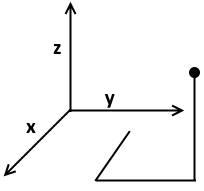
\includegraphics[width=4cm,height=5cm]{rysunki/wolne_x.png}
%   b)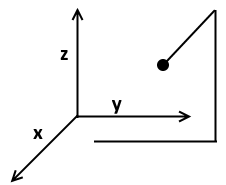
\includegraphics[width=4cm,height=5cm]{rysunki/wolne_y.png}
%   c)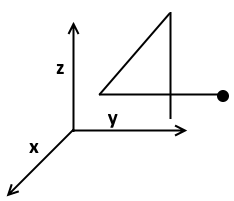
\includegraphics[width=4cm,height=5cm]{rysunki/wolne_z.png}
%   \caption{Nowo powstałe ścieżki w przypadku wolnych osi +x, +y lub +z}
%   \label{fig:nowe sciezki}
% \end{figure} 
% \\\indent Zajmiemy się teraz przypadkiem, w którym fragment ścieżki pomiędzy węzłami $v_i$ i $v_j$ nakłada się ze ścieżką łącząca $v_j$ z $v_j$ wzdłuż osi -z, dla \textit{k < i < j}. W takiej sytuacji przynajmniej jedna z osi -x lub -y musi być wolna. Jeżeli jest to oś -x zmieniamy ścieżkę zgodnie z rysunkiem \ref{fig:nakladanie}a, jeżeli -y wtedy musimy poprawić ścieżkę zgodnie z rysunkiem \ref{fig:nakladanie}b. Analogicznych operacji dokonamy jeżeli zajęta będzie oś -x lub -y.
% \begin{figure}[ht!]
%   \centering
%   a)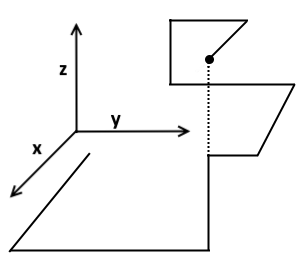
\includegraphics[width=6cm,height=5cm]{rysunki/zajete_z.png}
%   b)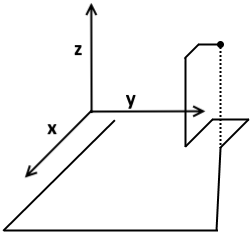
\includegraphics[width=6cm,height=5cm]{rysunki/zajete_z2.png}
%   \caption{Omijanie zajętej ścieżki w przypadku wolnej osi -x oraz -y}
%   \label{fig:nakladanie}
% \end{figure} 
% Tak powstała konstrukcja składa się z dziewięciu krawędzi. W przypadku, gdy zajdzie potrzeba ominięcia jeszcze jednej krawędzi uzyskamy ścieżkę składającą się z 15 odcinków.
% \todo{Rysunek?}
% \\\indent Po stworzeniu siatki wg powyższego przepisu uzyskamy w sumie \textit{e} krawędzi grafu \textit{G} składających się ze ścieżki $e_3$ złożonej z 3 odcinków, ścieżki $e_9$ z 9 odcinków oraz ścieżki $e_{15}$ z 15 odcinków co daje nam \textit{e = $e_3$ + $e_9$ + $e_{15}$}.

% \begin{Lemat}
% 	Pokrycie wierzchołkowe grafu \textnormal{G} o rozmiarze \textnormal{K} istnieje wtedy i tylko wtedy jeżeli istnieje pokrycie siatki \textnormal{P} wg powyższego algorytmu przez \textnormal{g = K + $e_3$ + 4$e_9$ + 7$e_{15}$} strażników.
% \end{Lemat}
% \textbf{Dowód.} Załóżmy, że istnieje pokrycie wierzchołkowe \textit{C} grafu \textit{G} o rozmiarze \textit{K}. Następnie, rozmieśćmy strażnika w każdym przecięciu siatki \textit{P} która odpowiada wierzchołkowi w \textit{C}.
% Niech $p_3$ będzie ścieżką złożoną z 3 odcinków w \textit{P} pomiędzy $v_i$ a $v_j$. Ponieważ \textit{C} jest pokryciem wierzchołkowym, przynajmniej w jednym z węzłów $v_i$ lub $v_j$ znajduje się strażnik a więc potrzebujemy jeszcze jednego strażnika aby strzec $p_3$. Podobna sytuacja występuje dla ścieżki $p_9$ pomiędzy $v_i$ oraz $v_j$. Jeden z węzłów $v_i$ lub $v_j$ jest już strzeżony więc dodatkowo potrzebujemy 4 strażników. Dla ścieżki $p_{15}$ potrzebujemy 7 dodatkowych strażników, co w rezultacie daje nam \textit{K + $e_3$ + 4$e_9$ + 7$e_{15}$} strażników.
% \\\indent Załóżmy teraz, że aby strzec siatkę \textit{P} wystarczy \textit{K + $e_3$ + 4$e_9$ + 7$e_{15}$} strażników. Każda z trzy elementowych ścieżek $e_3$ wymaga jednego strażnika w wewnętrznym rogu. Ścieżka złożona z dziewięciu odcinków wymaga czterech strażników rozmieszczonych w wewnętrznych rogach a piętnastowa odcinkowa - siedmiu. Stąd uzyskujemy sumę $e_3$ + 4$e_9$ + 7$e_{15}$ strażników rozmieszczonych w miejscach innych niż punkty siatki, którym odpowiadają wierzchołki grafu \textit{G}. Pozostało nam jeszcze \textit{K} strażników, których możemy umieścić tylko w punktach siatki odpowiadających wierzchołkom grafu \textit{G}. Załóżmy więc, że strażnicy rozmieszczeni w tych punktach nie należą do pokrycia wierzchołkowego \textit{G}. W takim wypadku krawędź \textit{(i, j)} z \textit{G} nie jest incydentna z żadnym wierzchołkiem należącym do pokrycia wierzchołkowego a więc odpowiadająca jej ścieżka w siatce \textit{P} nie posiada strażników zarówno w $v_i$ ani w $v_j$. Wiemy jednak, że aby pokryć np. ścieżkę trójelementową jeden strażnik w wewnętrznym rogu jest w stanie strzec tylko dwa z trzech odcinków. Analogiczna sytuacja występuje dla ścieżek o długości dziewięciu oraz piętnastu odcinków, w których, odpowiednio, czterech i siedmiu strażników jest w stanie strzec co najwyżej osiem i czternaście z dziewięciu oraz piętnastu odcinków. Stąd wnioskujemy, że jeżeli \textit{K} strażników nie stanowi pokrycia wierzchołkowego to nie możemy pokryć siatki \textit{P} przez \textit{K + $e_3$ + 4$e_9$ + 7$e_{15}$} strażników a więc \textit{K} strażników musi być pokryciem wierzchołkowym o rozmiarze co najwyżej \textit{K}.

% \begin{Twierdzenie}
% 	Zagadnienie strzeżenia trójwymiarowej siatki przez minimalną ilość strażników należy do klasy problemów NP-zupełnych.
% \end{Twierdzenie}
% \textbf{Dowód.} Ponieważ strażnicy mogą być rozmieszczeni tylko na skrzyżowania siatki lub w jej rogach, których jest skończona liczba rozwiązanie możemy zgadnąć oraz sprawdzić w czasie wielomianowym. Problem pokrycia wierzchołkowego należy do klasy NP-zupełnej a więc zagadnienie zredukowanie do tego problemu również należy do klasy NP-zupełnej.
\chapter{Problem pościgu i ucieczki w grafie}
\section{Gra w złodzieja i policjanta}
Mając dany graf \textit{G}, zbiór reguł \textit{S}, liczbę całkowita \textit{k}, oraz dwa warunki \textit{$T_1$, $T_2$}, gra zaczyna się od rozmieszczenia przez gracza pierwszego (policjanta) nie więcej niż \textit{k} żetonów na wierzchołkach grafu \textit{G}. Gracz numer dwa (złodziej) rozmieszcza jeden żeton na dowolnym wierzchołku \textit{G}. Następnie gracze przesuwają swoje żetony, zgodnie z regułami \textit{S}, dopóki nie zajdzie jeden z warunków $T_i$. Jeżeli końcowa konfiguracja spełnia warunek $T_1$ - wygrywa policjant, w przeciwnym wypadku wygrywa złodziej. W klasycznej wersji gry, obaj gracze znają rozmieszczenie wszystkich żetonów a jedynym warunkiem końcowym jest aby żeton gracza pierwszego oraz drugiego znajdował się na tym samym wierzchołku grafu G.
Reguły \textit{S} wyglądają następująco:
\begin{enumerate}
  \item Gracze wykonują ruchy na przemian
  \item Gracz pierwszy w swojej kolejce może odmówić ruchu lub przesunąć wzdłuż krawędzi jeden ze swoich żetonów na wierzchołek sąsiedni z aktualnie zajmowanym
  \item Gracz drugi w swojej kolecje może odmówić ruchu lub przesunąć wzdłuż krawędzi swój żeton na wolny wierzchołek, sąsiedni z wierzchołkiem aktualnie zajmowanym
\end{enumerate}

Problem ma praktyczne zastosowanie na przykład w planowaniu ruchu robotów, kiedy ważnym jest aby nie następowały kolizje lub poważniejsze zderzenia.

Zagadnienie pościgu i ucieczki w grafie, opiera się na przeszukiwaniu grafu w taki sposób aby po wykonaniu \textit{n} kroków, policjant zauważył złodzieja (tzn. znajdował się w tym samym wierszu lub w tej samej kolumnie) lub, w trudniejszym wariancie, znajdował się w tym samym wierzchołku co złodziej. Taką sytuację uznajemy za zwycięstwo goniącego, w przeciwnym wypadku zwycięża złodziej. Obaj uczestnicy poruszają się tylko po wierszach i kolumnach siatki z ograniczoną prędkością.

% \begin{figure}[ht!]
%   \centering
%   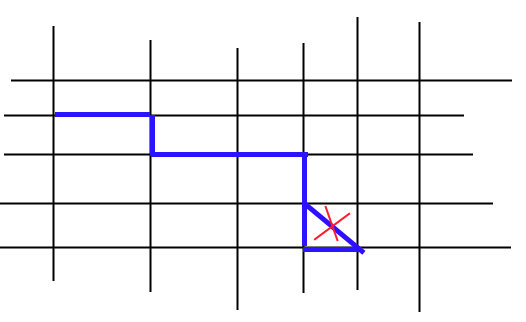
\includegraphics{rysunki/przykladowy_ruch.png}
%   \caption{Przykładowy ruch po siatce}
% \end{figure} 
% \todo{Poprawić rysunek}
Najprostszym przykładem gry, w której zawsze zwycięża policjant jest drzewo oraz współczynnik k = 1. W takim przypadku policjant w każdym kolejnym ruchu zbliża się do drugiego gracza, który w żadnym momencie nie jest w stanie go minąć, co zawsze prowadzi do zwycięstwa goniącego.

\subsection{Wariant Sugiharu i Suzuki}
W tym rozdziale zajmę się innym wariantem gry, przedstawionym przez Sugiharu i Suzuki, w którym warunkiem zwycięstwa policjanta jest zauważenie złodzieja a gra odbywa się na grafie \textit{G} przypominającym prostokątną siatkę.
Przez siatkę rozumiemy graf \textit{$G_{n,m}$}, gdzie \textit{n} to liczba wierzchołków a \textit{m} liczba krawędzi, z których każda ma długość jeden. Zakładamy również, że graf jest rozpięty na płaszczyźnie z punktem poczatkowym \textit{$v_{0,0}$} w lewym górnym wierzchołku.
\begin{Definicja}
  Gracz A \textnormal{jest widoczny} dla gracza B wtedy i tylko wtedy, gdy obaj znajdują się w tej samej kolumnie lub w tym samym wierszu siatki, niezależnie od odległości która ich dzieli.
\end{Definicja}

Gracz przesuwają swoje żetony tylko po krawędziach grafu a szybkość ruchu jest określona przed rozpoczęciem gry.
W tym wariancie gry, gracze nie mają całkowitej wiedzy o pozycjach, które zajmują. Tylko złodziej posiada wszystkie informacje o miejscach, które zajmuje policjant. Ścigający za to nie wie nic o pozycji uciekającego, dopóki nie zostanie on zauważony. Dodatkowo, ruchy pierwszego gracza są z góry określone, zanim gra w ogóle się rozpocznie.
Zasady \textit{S} wyglądają następująco:
\begin{enumerate}
  \item Gracze poruszają się w czasie rzeczywistym
  \item Prędkość ścigającego jest stała i wynosi $s_n$
  \item Uciekający porusza się z prędkością co najwyżej $s_c$
\end{enumerate}

Warunki kończące grę:
\begin{enumerate}
  \item Złodziej został zauważony przez policjanta
  \item Uciekający zawsze jest w stanie zapobiec zwycięstwu policjanta
\end{enumerate}

Podobnie jak zwykły problem gonitwy i ucieczki, również ta odmiana jest całkowicie deterministyczna i zależy od parametrów początkowych gry. Naszym celem jest określenie warunków, w których zawsze zwycięża gracz pierwszy. 

\begin{Twierdzenie}
	Jeżeli $S_n$ $\le$ n + 1, policjant zawsze wygrywa dla stałej $S_c$ = n + 1.
\end{Twierdzenie}
\textbf{Dowód.} Aby dowieść powyższego twierdzenia skorzystamy z następującego algorytmu
\begin{enumerate}
	\item Gracz pierwszy porusza się w dół kolumną \textit{j}, startując w wierzchołku \textit{(0,j)}, przechodząc przez wierzchołek \textit{(n, j)} a kończąc ruch w \textit{(n, j + 1)}. Pokonanie takiej trasy zajmuje jedną jednostkę czasu.
	\item Następnie, przesuwa się w górę kolumną \textit{j + 1}, kończąc ruch w wierzchołku \textit{(0,j)}. Pokonanie takiej ścieżki również zajmuje jedną jednostkę czasu.
	\item Powtarzamy ruch nr 1
	\item Wykonuje ruch w górę kolumną \textit{j + 1}, kończąc go w wierzchołku \textit{(0,j + 1)}, tracąc $\frac{n}{n+1}$ jednostki czasu.
\end{enumerate}
\begin{figure}[ht!]
  \centering
  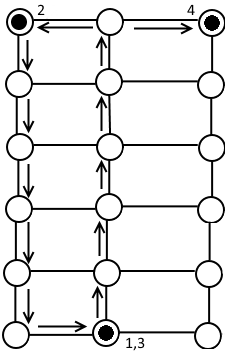
\includegraphics[height=2cm]{rysunki/schemat_ruchu.png}
  \caption{Trasa pokonana przez gracza pierwszego w wyniku algorytmu}
  \todo[inline]{Poprawić ten obrazek}
\end{figure} 

Czas, którego potrzebował gracz pierwszy aby wykonać powyższy schemat wynosi $t_{j+1}$ = $t_j$ + 3 + $\frac{n}{n+1}$.
Zakładamy, że po wykonaniu powyższych ruchów, gracz numer dwa albo został już zauważony, co kończy grę, lub znajduje się w części siatki ograniczonej przez wierzchołki [(0,0), (n, j + 1)].
\indent Jako, że gra toczy się dalej, gracz numer dwa nie może znajdować się w pierwszym wierszu ani \textit{j-tej} kolumnie ponieważ wtedy byłby widoczny dla policjanta. W czasie \textit{$t_j$} drugi gracz znajduje się w części siatki ograniczonej przez wierzchołki [(0,j), (n, j + 1)] i próbuje się przedostać do części [(0,0), (n, j + 1)]

\begin{figure}[ht!]
  \centering
  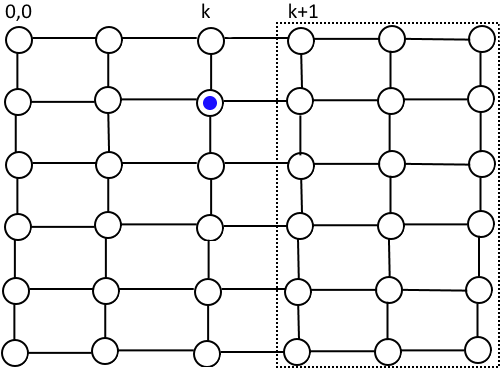
\includegraphics[height=5cm]{rysunki/podsiatka.png}
  \caption{Złodziej znajduje się w części siatki zaznaczonej linią przerywaną}
\end{figure} 

\indent W czasie, kiedy policjant przemieszcza się kolumną \textit{j}, złodziej może zbliżać się do niej wierszem \textit{i}. Policjant dotrze do wierzchołka (i,j) po czasie $\frac{i}{n+1}$ a więc do tego momentu złodziej musi znajdować się powyżej (lub poniżej) wiersza \textit{i}. Wynika z tego, że w momencie kiedy gracz nr jeden kończy pierwszy ruch, drugi gracz znajduje się w odległości $\frac{1-i}{n+1}$ - $\epsilon$ pomiędzy kolumną (i,j + 1) a kolumną (i,j). Obrazuje to rysunek \ref{fig:pierwszy krok}.
\begin{figure}[ht!]
  \centering
  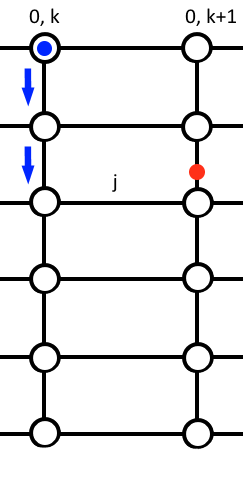
\includegraphics[width=5cm,height=2cm]{rysunki/poscig_1.png}
  \caption{Pierwszy etap pościgu.}
  \label{fig:pierwszy krok}
\end{figure}
\\\indent Pierwszy gracz ponownie przekroczy wiersz \textit{i} w drugim kroku algorytmy po upływie $\frac{n-1}{n+1}$ czasu. Do tego momentu, drugi gracz musi przejść cały wiersz i znaleźć się w kolumnie \textit{j}. Żeby tego dokonać musi przemieścić się o $\frac{i}{n+1}$ + $\delta$ w ciągu $\frac{n-1}{n+1}$ jednostek czasu. Daje nam to ograniczenie \textit{i < $\frac{n}{2}$}.
\\\indent Pomiędzy momentem kiedy policjant przekracza wiersz \textit{i} w kroku drugim a przejściem do wierzchołka (0,j) mija $\frac{i}{n+1}$ jednostki czasu. W sumie mijają dwie jednostki czasu od momentu $t_j$. Złodziej startując w kolumnie \textit{j + 1} i poruszając się wzdłuż wiersza \textit{i} nie ma wystarczajaco dużo czasu aby przesunąć się do wiersza \textit{i - 1} lub \textit{i + 1} ponieważ nie może rozpocząć ruchu dopóki pierwszy gracz nie przekroczy wiersza \textit{i}. Więc w momencie, kiedy ścigający kończy ruch nr dwa, drugi gracz musi znajdować się w odległości nie większej niż $\frac{i}{n+1}$ - $\gamma$ od (i,j). Jako, że \textit{i < $\frac{n}{2}$}.
\begin{center}
$\frac{i}{n+1}$ - $\gamma$ < 1 - $\frac{i}{n+1}$
\end{center}
Widać to na rysunku \ref{fig:fig:drugi krok}.
\begin{figure}[ht!]
  \centering
  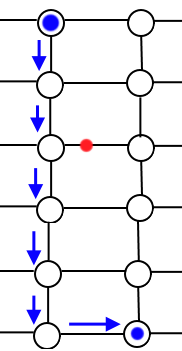
\includegraphics[width=5cm,height=5cm]{rysunki/poscig_2.png}
  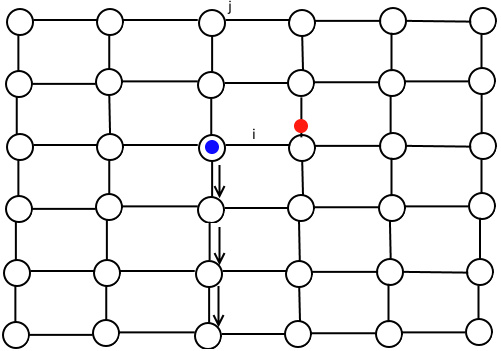
\includegraphics[width=5cm,height=5cm]{rysunki/poscig_3.png}
  \caption{Drugi etap pościgu}
  \label{fig:drugi krok}
\end{figure}

\indent Pierwszy gracz osiąga (i,j) w kroku trzecim po upływie kolejnych $\frac{i}{n+1}$ jednostek. W tym samym czasie drugi gracz nie jest w stanie osiągnąć kolumny \textit{j - 1} ani wrócić do \textit{j + 1} a więc zostaje zauważony.
\begin{figure}[ht!]
  \centering
  \includegraphics[width=5cm,height=5cm]{rysunki/poscig_4.png}
  \includegraphics[width=5cm,height=5cm]{rysunki/poscig_5.png}
  \caption{Ostatni etap pościgu.}
  \label{fig:ostatni etap poscigu}
\end{figure} 


\indent Ponieważ policjant widzi przez całą długość wiersza/kolumny, takie samo rozumowanie będzie miało zastosowanie jeżeli złodziej będzie rozpoczynał swój ruch z każdej kolumny \textit{k > j + 1}. W ten sposób jeżeli pierwszy gracz rozpocznie grę w punkcie (0,0) oraz wszystkie założenia początkowe będą spełnione zawsze zakończy grę sukcesem w czasie nie większym niż \textit{$t_n$}.



% % %\summary
% % %
% % %Streszczenie…

% % % załączniki (opcjonalnie):
% \appendix
% \chapter{Triangulacja wielokąta}\label{triangulacja}
% \begin{Lemat}\label{podzial na trojkaty}
% N-kąt prosty można zawsze podzielić na n-2 trójkątów.
% \end{Lemat}
% Dowód przez indukcję po n:
% \\Jeżeli n = 3 wielokąt jest już podzielony.
% Załóżmy, że n $\ge$ 3 i rozpatrzmy skrajny lewy wierzchołek \textit{v} oraz jego sąsiadów \textit{u}, \textit{w}.
% W pierwszym przypadku odcinek \textit{uw} jest przekątną a w drugim część krawędzi wielokąta P leży wewnątrz trójkąta \textit{uvw}.
% \begin{align*}
% \includegraphics[height=5cm]{rysunki/triangulacja_1.png} \hspace{3cm} \includegraphics[height=5cm]{rysunki/triangulacja_2.png}
% \end{align*}
% \\\indent W pierwszym przypadku przekątna $\overline{u w}$ dzieli wielokąt na trójkąt oraz wielokąt prosty o n-1 wierzchołkach, na którym wykonujemy kolejny krok indukcji.
% \\\indent W przypadku drugim znajdujemy punkt \textit{t}, który znajduje się najdalej od prostej \textit{uw} a następnie łączymy go z punktem \textit{v}. Odcinek $\overline{v t}$ musi być przekątną, która dzieli wielokąt na dwa proste wielokąty o \textit{m} oraz \textit{n - m + 2} wierzchołkach, gdzie \textit{3 $\ge$ m $\ge$ n-1} na którym wykonujemy kolejny krok indukcji.
% \\\indent Na mocy lematu \ref{podzial na trojkaty} tak podzielony wielokąt możemy triangulować przy użyciu \textit{m - 2 + n - m + 2 - 2 = n - 2} trójkątów

% %Załącznik…
% %
% %\chapter{Tytuł załącznika}
% %
% %Załącznik…
% \begin{bibdiv}
% \begin{biblist}

%  \bibselect{literatura}
%   Joseph O'Rourke - Art gallery theorems and algorithms
%  \\*Journal of Combinatorial Theory 18, 39-41 (1975)
%  \\*Aldo Laurentini - Guardin the walls of an art gallery (The Visual Computer, 1999)
%  \\*. J. Czyzowicz, E. Rivera-Campo, N. Santoro, J. Urrutia, and J. Zaks. Guarding rectangular art galleries. Discrete Applied Math, 50:149–157, 1994. 

% \end{biblist}
% \end{bibdiv}

% spis tabel
% \listoftables

% spis rysunków
% \listoffigures

% \oswiadczenie

\end{document}